%  LaTeX support: latex@mdpi.com 
%  For support, please attach all files needed for compiling as well as the log file, and specify your operating system, LaTeX version, and LaTeX editor.

%=================================================================
\documentclass[sensors,article,submit,pdftex,moreauthors]{Definitions/mdpi} 
% For posting an early version of this manuscript as a preprint, you may use "preprints" as the journal and change "submit" to "accept". The document class line would be, e.g., \documentclass[preprints,article,accept,moreauthors,pdftex]{mdpi}. This is especially recommended for submission to arXiv, where line numbers should be removed before posting. For preprints.org, the editorial staff will make this change immediately prior to posting.

%--------------------
% Class Options:
%--------------------
%----------
% journal
%----------
% Choose between the following MDPI journals:
% acoustics, actuators, addictions, admsci, adolescents, aerospace, agriculture, agriengineering, agronomy, ai, algorithms, allergies, alloys, analytica, animals, antibiotics, antibodies, antioxidants, applbiosci, appliedchem, appliedmath, applmech, applmicrobiol, applnano, applsci, aquacj, architecture, arts, asc, asi, astronomy, atmosphere, atoms, audiolres, automation, axioms, bacteria, batteries, bdcc, behavsci, beverages, biochem, bioengineering, biologics, biology, biomass, biomechanics, biomed, biomedicines, biomedinformatics, biomimetics, biomolecules, biophysica, biosensors, biotech, birds, bloods, blsf, brainsci, breath, buildings, businesses, cancers, carbon, cardiogenetics, catalysts, cells, ceramics, challenges, chemengineering, chemistry, chemosensors, chemproc, children, chips, cimb, civileng, cleantechnol, climate, clinpract, clockssleep, cmd, coasts, coatings, colloids, colorants, commodities, compounds, computation, computers, condensedmatter, conservation, constrmater, cosmetics, covid, crops, cryptography, crystals, csmf, ctn, curroncol, currophthalmol, cyber, dairy, data, dentistry, dermato, dermatopathology, designs, diabetology, diagnostics, dietetics, digital, disabilities, diseases, diversity, dna, drones, dynamics, earth, ebj, ecologies, econometrics, economies, education, ejihpe, electricity, electrochem, electronicmat, electronics, encyclopedia, endocrines, energies, eng, engproc, ent, entomology, entropy, environments, environsciproc, epidemiologia, epigenomes, est, fermentation, fibers, fintech, fire, fishes, fluids, foods, forecasting, forensicsci, forests, foundations, fractalfract, fuels, futureinternet, futureparasites, futurepharmacol, futurephys, futuretransp, galaxies, games, gases, gastroent, gastrointestdisord, gels, genealogy, genes, geographies, geohazards, geomatics, geosciences, geotechnics, geriatrics, hazardousmatters, healthcare, hearts, hemato, heritage, highthroughput, histories, horticulturae, humanities, humans, hydrobiology, hydrogen, hydrology, hygiene, idr, ijerph, ijfs, ijgi, ijms, ijns, ijtm, ijtpp, immuno, informatics, information, infrastructures, inorganics, insects, instruments, inventions, iot, j, jal, jcdd, jcm, jcp, jcs, jdb, jeta, jfb, jfmk, jimaging, jintelligence, jlpea, jmmp, jmp, jmse, jne, jnt, jof, joitmc, jor, journalmedia, jox, jpm, jrfm, jsan, jtaer, jzbg, kidney, kidneydial, knowledge, land, languages, laws, life, liquids, literature, livers, logics, logistics, lubricants, lymphatics, machines, macromol, magnetism, magnetochemistry, make, marinedrugs, materials, materproc, mathematics, mca, measurements, medicina, medicines, medsci, membranes, merits, metabolites, metals, meteorology, methane, metrology, micro, microarrays, microbiolres, micromachines, microorganisms, microplastics, minerals, mining, modelling, molbank, molecules, mps, msf, mti, muscles, nanoenergyadv, nanomanufacturing, nanomaterials, ncrna, network, neuroglia, neurolint, neurosci, nitrogen, notspecified, nri, nursrep, nutraceuticals, nutrients, obesities, oceans, ohbm, onco, oncopathology, optics, oral, organics, organoids, osteology, oxygen, parasites, parasitologia, particles, pathogens, pathophysiology, pediatrrep, pharmaceuticals, pharmaceutics, pharmacoepidemiology, pharmacy, philosophies, photochem, photonics, phycology, physchem, physics, physiologia, plants, plasma, pollutants, polymers, polysaccharides, poultry, powders, preprints, proceedings, processes, prosthesis, proteomes, psf, psych, psychiatryint, psychoactives, publications, quantumrep, quaternary, qubs, radiation, reactions, recycling, regeneration, religions, remotesensing, reports, reprodmed, resources, rheumato, risks, robotics, ruminants, safety, sci, scipharm, seeds, sensors, separations, sexes, signals, sinusitis, skins, smartcities, sna, societies, socsci, software, soilsystems, solar, solids, sports, standards, stats, stresses, surfaces, surgeries, suschem, sustainability, symmetry, synbio, systems, taxonomy, technologies, telecom, test, textiles, thalassrep, thermo, tomography, tourismhosp, toxics, toxins, transplantology, transportation, traumacare, traumas, tropicalmed, universe, urbansci, uro, vaccines, vehicles, venereology, vetsci, vibration, viruses, vision, waste, water, wem, wevj, wind, women, world, youth, zoonoticdis 

%---------
% article
%---------
% The default type of manuscript is "article", but can be replaced by: 
% abstract, addendum, article, book, bookreview, briefreport, casereport, comment, commentary, communication, conferenceproceedings, correction, conferencereport, entry, expressionofconcern, extendedabstract, datadescriptor, editorial, essay, erratum, hypothesis, interestingimage, obituary, opinion, projectreport, reply, retraction, review, perspective, protocol, shortnote, studyprotocol, systematicreview, supfile, technicalnote, viewpoint, guidelines, registeredreport, tutorial
% supfile = supplementary materials

%----------
% submit
%----------
% The class option "submit" will be changed to "accept" by the Editorial Office when the paper is accepted. This will only make changes to the frontpage (e.g., the logo of the journal will get visible), the headings, and the copyright information. Also, line numbering will be removed. Journal info and pagination for accepted papers will also be assigned by the Editorial Office.

%------------------
% moreauthors
%------------------
% If there is only one author the class option oneauthor should be used. Otherwise use the class option moreauthors.

%---------
% pdftex
%---------
% The option pdftex is for use with pdfLaTeX. If eps figures are used, remove the option pdftex and use LaTeX and dvi2pdf.

%=================================================================
% MDPI internal commands
\firstpage{1} 
\makeatletter 
\setcounter{page}{\@firstpage} 
\makeatother
\pubvolume{1}
\issuenum{1}
\articlenumber{0}
\pubyear{2022}
\copyrightyear{2022}
%\externaleditor{Academic Editor: Firstname Lastname}
\datereceived{} 
%\daterevised{} % Only for the journal Acoustics
\dateaccepted{} 
\datepublished{} 
%\datecorrected{} % Corrected papers include a "Corrected: XXX" date in the original paper.
%\dateretracted{} % Corrected papers include a "Retracted: XXX" date in the original paper.
\hreflink{https://doi.org/} % If needed use \linebreak
%\doinum{}
%------------------------------------------------------------------
% The following line should be uncommented if the LaTeX file is uploaded to arXiv.org
%\pdfoutput=1

%=================================================================
% Add packages and commands here. The following packages are loaded in our class file: fontenc, inputenc, calc, indentfirst, fancyhdr, graphicx, epstopdf, lastpage, ifthen, lineno, float, amsmath, setspace, enumitem, mathpazo, booktabs, titlesec, etoolbox, tabto, xcolor, soul, multirow, microtype, tikz, totcount, changepage, attrib, upgreek, cleveref, amsthm, hyphenat, natbib, hyperref, footmisc, url, geometry, newfloat, caption
\usepackage{makecell}
\usepackage{placeins}
\usepackage{amsmath}
\usepackage{comment}
\usepackage{soulutf8}
\usepackage[adjustmargins]{LatexPackage/trackchanges}
\addeditor{H.K.D}

%=================================================================
%% Please use the following mathematics environments: Theorem, Lemma, Corollary, Proposition, Characterization, Property, Problem, Example, ExamplesandDefinitions, Hypothesis, Remark, Definition, Notation, Assumption
%% For proofs, please use the proof environment (the amsthm package is loaded by the MDPI class).

%=================================================================
% Full title of the paper (Capitalized)
\Title{SKIN LESION CLASSIFICATION ON IMBALANCED DATA USING DEEP LEARNING WITH SOFT ATTENTION}

% MDPI internal command: Title for citation in the left column
\TitleCitation{SKIN LESION CLASSIFICATION ON IMBALANCED DATA USING DEEP LEARNING WITH SOFT ATTENTION}

% Author Orchid ID: enter ID or remove command
\newcommand{\orcidauthorA}{0000-0001-7152-0191} % Add \orcidA{} behind the author's name
\newcommand{\orcidauthorB}{0000-0001-9934-7474} % Add \orcidB{} behind the author's name
\newcommand{\orcidauthorC}{0000-0002-2566-5637} % Add \orcidC{} behind the author's name

% Authors, for the paper (add full first names)
\Author{Viet Dung Nguyen $^{1,\dagger, *}$\orcidA{}, Ngoc Dung Bui $^{2,\dagger}$\orcidB and Hoang Khoi Do  $^{1,\dagger}$\orcidC{}}

%\longauthorlist{yes}

% MDPI internal command: Authors, for metadata in PDF
\AuthorNames{Viet Dung Nguyen, Ngoc Dung Bui and Hoang Khoi Do}

% MDPI internal command: Authors, for citation in the left column
\AuthorCitation{Nguyen, V.D.; Bui, N.D.; Do, H.K.}
% If this is a Chicago style journal: Lastname, Firstname, Firstname Lastname, and Firstname Lastname.

% Affiliations / Addresses (Add [1] after \address if there is only one affiliation.)

\address{
$^{1}$ \quad School of Electrical and Electronic Engineering, Hanoi University of Science and Technology, Vietnam; dung.nguyenviet1@hust.edu.vn\\
$^{2}$ \quad Faculty of Information Technology, University of Transport and Communications, Vietnam; dnbui@utc.edu.vn\\
$^{3}$ \quad School of Electrical and Electronic Engineering, Hanoi University of Science and Technology, Vietnam; khoi.dh200322@sis.hust.edu.vn}

% Contact information of the corresponding author
\corres{Correspondence: dung.nguyenviet1@hust.edu.vn; Tel.:  +84-9834-443-22 (N.V.D.)}

% Current address and/or shared authorship
\firstnote{Current address: 1st Dai Co Viet Street, Ha Noi, Vietnam} 
% The commands \thirdnote{} till \eighthnote{} are available for further notes 

%\simplesumm{} % Simple summary

%\conference{} % An extended version of a conference paper

% Abstract (Do not insert blank lines, i.e. \\) s
\abstract{Today, the rapid development of industrial zones leads to an increased incidence of skin	diseases because of polluted air. According to a report by the American Cancer Society, it is estimated that in 2022 there will be about 100,000 people suffering from skin cancer and more than 7600 of these people will not survive. In the context that doctors at provincial hospitals and health facilities are overloaded, doctors at lower levels lack experience and having	a tool to support doctors in the process of diagnosing skin diseases quickly and accurately is essential. Along with the strong development of artificial intelligence technologies, many solutions to support the diagnosis of skin diseases have been researched and developed. In this paper, a combination of \add[H.K.D]{one} SOTA model \change[H.K.D]{such as}{including} DenseNet, InceptionNet, ResNet, NasNet,  MobileNet and Soft-Attention is proposed. Furthermore, personal information including age and gender are also used. It is worth to note that a new loss function	that takes into account the data imbalance is also proposed. Experimental results on data set HAM10000 show that using InceptionResNetV2 with Soft-Attention and new loss function gives 90 percent accuracy, mean of precision, f1-score, recall-score, and AUC scores of 0.81, 0.81, 0.82, and 0.99, respectively. Besides, using MobileNetV3Large combined with Soft-Attention and new loss function, even though the number of parameters is 11 times less, the number of hidden layers is 4 times less, it achieves 0.86 accuracy and 30 times faster diagnosis than InceptionResNetV2.}

% Keywords
\keyword{Skin Lesions, Classification, Deep Learning, Soft-Attention, Imbalance} 

% The fields PACS, MSC, and JEL may be left empty or commented out if not applicable
%\PACS{J0101}
%\MSC{}
%\JEL{}

%%%%%%%%%%%%%%%%%%%%%%%%%%%%%%%%%%%%%%%%%%
% Only for the journal Diversity
%\LSID{\url{http://}}

%%%%%%%%%%%%%%%%%%%%%%%%%%%%%%%%%%%%%%%%%%
% Only for the journal Applied Sciences
%\featuredapplication{Authors are encouraged to provide a concise description of the specific application or a potential application of the work. This section is not mandatory.}
%%%%%%%%%%%%%%%%%%%%%%%%%%%%%%%%%%%%%%%%%%

%%%%%%%%%%%%%%%%%%%%%%%%%%%%%%%%%%%%%%%%%%
% Only for the journal Data
%\dataset{DOI number or link to the deposited data set if the data set is published separately. If the data set shall be published as a supplement to this paper, this field will be filled by the journal editors. In this case, please submit the data set as a supplement.}
%\datasetlicense{License under which the data set is made available (CC0, CC-BY, CC-BY-SA, CC-BY-NC, etc.)}

%%%%%%%%%%%%%%%%%%%%%%%%%%%%%%%%%%%%%%%%%%
% Only for the journal Toxins
%\keycontribution{The breakthroughs or highlights of the manuscript. Authors can write one or two sentences to describe the most important part of the paper.}

%%%%%%%%%%%%%%%%%%%%%%%%%%%%%%%%%%%%%%%%%%
% Only for the journal Encyclopedia
%\encyclopediadef{For entry manuscripts only: please provide a brief overview of the entry title instead of an abstract.}

%%%%%%%%%%%%%%%%%%%%%%%%%%%%%%%%%%%%%%%%%%
\begin{document}

%%%%%%%%%%%%%%%%%%%%%%%%%%%%%%%%%%%%%%%%%%
\setcounter{section}{0} %% Remove this when starting to work on the template.
\begin{comment}
	\section{How to Use this Template}
	
	The template details the sections that can be used in a manuscript. Note that the order and names of article sections may differ from the requirements of the journal (e.g., the positioning of the Materials and Methods section). Please check the instructions on the authors' page of the journal to verify the correct order and names. For any questions, please contact the editorial office of the journal or support@mdpi.com. For LaTeX-related questions please contact latex@mdpi.com.%\endnote{This is an endnote.} % To use endnotes, please un-comment \printendnotes below (before References). Only journal Laws uses \footnote.
	
	% The order of the section titles is: Introduction, Materials and Methods, Results, Discussion, Conclusions for these journals: aerospace,algorithms,antibodies,antioxidants,atmosphere,axioms,biomedicines,carbon,crystals,designs,diagnostics,environments,fermentation,fluids,forests,fractalfract,informatics,information,inventions,jfmk,jrfm,lubricants,neonatalscreening,neuroglia,particles,pharmaceutics,polymers,processes,technologies,viruses,vision
\end{comment}

\section{Introduction} 
\subsection{Problem Statement}
\change[H.K.D]{One of the most common malignancies that cause death globally is skin cancer. In the United States, more than 9500 persons receive a skin cancer diagnosis each day \mbox{\cite{03358}}. The Skin Cancer Foundation reports that there is an ongoing rise in the incidence of skin cancer worldwide \mbox{\cite{11872}}. In the United States, 192,310 new cases of melanoma are anticipated to be detected in 2019. On the other hand, if patients receive an early diagnosis, their chances of survival are 99 percent. Survival is, however, generally poor after the illness has spread beyond the skin \mbox{\cite{11872}}. Additionally, there is a need for an efficient solution because to the rising prevalence of skin malignancies, low awareness among a population that is expanding, and a lack of sufficient clinical competence and services.}{Skin cancer is one of the most common cancers leading to worldwide death. Every day, more than 9500 \mbox{\cite{03358}} people in the United States are diagnosed with skin cancer. Otherwise, 3.6 \mbox{\cite{03358}} million people are diagnosed with basal cell skin cancer each year. According to the Skin Cancer Foundation, the global incidence of skin cancer continues to increase \mbox{\cite{11872}}. In 2019, it is estimated that 192,310 cases of melanoma will be diagnosed in the United States \mbox{\cite{11872}}. On the other hand, if patients are early diagnosed, the survival rate is correlated with 99 percent. However, once the disease progresses beyond the skin, survival is poor \mbox{\cite{11872}}. Moreover, with the increasing incidence of skin cancers, low awareness among a growing population, and a lack of adequate clinical expertise and services, there is a need for effective solution.} 

Recently, deep learning particularly, and machine learning in general algorithms have emerged to achieve excellent performance on various tasks, especially in skin disease diagnosis tasks. AI-enabled computer-aided diagnostics (CAD) has solutions in three main categories: Diagnosis, Prognosis, and Medical Treatment. Medical imaging, including ultrasound, computed tomography, magnetic resonance imaging, and X-ray image is used extensively in clinical practice. In Diagnosis, Artificial Intelligence (AI) algorithms are applied for disease detection to save progress execution before these diagnosis results are considered by a doctor. In Prognosis, AI algorithms are used to predict the survival rate of a patient based on his/her history and medical data. In Medical Treatment, AI models are applied to build solutions to a specific disease, medicine revolution is an example. In various studies, AI algorithms have provided various end-to-end solutions to the detection of abnormalities such as breast cancer, brain tumors, lung cancer, esophageal cancer, skin lesions, and foot ulcers across multiple image modalities of medical imaging \cite{11872}.

To adapt the rise in skin cancer case, AI algorithms over the last decade has a great performance. Some typical models that can be mentioned are DenseNet \cite{06993}, EfficientNet \cite{04861}, Inception \cite{00567}, MobileNets\cite{04861}\cite{04381}\cite{02244}, ResNet \cite{03385} \cite{05027}, and NasNet \cite{07012}. Some of these models which have been used as a backbone model in this paper will be discussed in the Related Work section.

\subsection{Related Works}
\change[H.K.D]{Skin lesion classification is not a new area, since there are many great performance models constructed. One of the most cutting-edge technologies that have been used is Soft-Attention as stated in \mbox{\cite{03358}}. Soumyyak et al construct several models formed by the combination of a backbone model including DenseNet201 \mbox{\cite{06993}}, InceptionResNetV2 \mbox{\cite{00567}}, ResNet50 \mbox{\cite{03385} \cite{05027}}, VGG16 \mbox{\cite{1556}} and Soft-Attention layer. Their approach is to add the Soft-Attention layer at the end or the middle of the backbone model. For ResNet50 and VGG16, the Soft-Attention layer is added after the third residual block and CNN block, respectively. DenseNet201 and InceptionResNetV2, otherwise concatenate with the Soft-Attention before a fully-connected layer, and then soft-max layer.
	
Using those above backbones has been tried by many previous papers. Rishu Garg et al \mbox{\cite{03798}} uses transfer learning approach with CNN based model: ResNet50 and VGG16 which are pretrained with ImageNet data set. Besides, they also use data augmentation to avoid the imbalance of the data set. Histogram Equalization is also used to increase the contrast of the skin lesions before feeding into the Machine Learning algorithms including Random Forest, XGBoost, Support Vector Machine.	
	
Amirreaza et al \mbox{\cite{10348}} do not only use those above backbone model but also used InceptionV3 \mbox{\cite{00567}} model. In that research, the dataset HAM10000 and $PH^2$ are combined to create a 8 classes data set. Before feeding into the Deep CNN models, the image is resized to (224, 224) for DenseNet201, ResNet152, InceptionResNetV2 and (229, 229) for InceptionV3. 
	
Another paper that uses the backbone models is \mbox{\cite{09418}}, Hemanth et al decide to use EfficientNet \mbox{\cite{11946}} and SeNET \mbox{\cite{01507}} instead and CutOut \mbox{\cite{04552v2}} method which involves creating holes of different sizes on the images i.e. technically making a random portion of image inactive during data augmentation process. 
	
Otherwise, \mbox{\cite{01284}} also used Deep Convolution Neural Network, Peng Yao et al used RandArgument which crops an image into several images from a fixed size, DropBlock which is used for regularization, Multi-Weighted New Loss which is used for dealing with the imbalanced data problem, end-to-end Cumulative Learning Strategy which can more effectively balance representation learning and classifier learning without additional computational cost. 
	
Another state of the art is GradCam and Kernel SHAP \mbox{\cite{06612}}, Kyle Young et al create model agnostic, local interpretable methods that can highlight pixels that the trained network deems relevant for the final classification. In that research they use three data sets containing HAM10000, BCN-20000 and MSK. Before feeding into the models, the images are preprocessed by binarized with a very low threshold to find the center of mass. 
	
On the other hand, there are also many state of the art whose great performance on skin lesion classification. The Student and Teacher Model is also a high performance model in 2021 \mbox{\cite{03225}}, which is created by Xiaohan Xing et al as the combination of two model which share the memory with each other. Therefore, they can take full advantage of what others learn. 

SkinLinkNet \mbox{\cite{12602}} and WonderM \mbox{\cite{03426}} are both tested the effect of segmentation on skin lesion classification problem created by Amirreza et al and Yeong Chan et al, respectively. In WonderM, the method used is padding the image so that the image has the shape increased from (450, 600) to (600, 600). In SkinLinkNet, instead resize the image down to (448, 448). Both of SkinLinkNet and WonderM use UNet to do the segmentation task, though they use EfficientNetB0 and DenseNet to do the classification task, respectively. 
	
Another approach is using metadata including gender, age, and capturing position as stated in \mbox{\cite{03910}} by Nil Gessert et al. The metadata is fed into fully connected neural network after being encoded into one-hot vector. All missing data point of age is set to 0. To overcome the missing data problem, the research apply one-hot encoding to the group but the initial validation is poor performance then numerical encoding is applied.
	
On the other hand, skin lesion classification problems are not only applied by Deep Learning but also Machine Learning. Random Forest, XGBoost, and Support Vector Machines are tested by \mbox{\cite{03798}} of Rishu Garg et al. Besides, Isolation Forest is applied before the soft-max activation of the deep learning model to detect out of distribution skin lesion images as stated in \mbox{\cite{10348}} by Amirreza Rezvantalab et al. Matrix Transformation, besides is also applied before the soft-max activation function in \mbox{\cite{05045}} by Michele Alberti et al.}

{Skin lesion classification is not a new area, since there are many great performance models constructed, recent years. The skin classification approaches can be divided into two main approaches: Deep Learning and Machine Learning. Both approaches gain great performance. Data Augmentation and Feature Extractor, otherwise are two main supporters that make the model better.
\begin{table}[H]
	\centering
	\begin{tabular}{| c | p{1.5cm} | p{1.5cm} | p{2cm} | p{1.5cm} | p{2cm} | p{1cm} |}
		\hline
		Work & Deep Learning & Machine Learning & Data 
		Augmentation & Feature Extractor & Data set & Result\\
		\hline
		\cite{03358} & Classify & & x & & HAM10000 & 0.93 (ACC)\\
		\hline
		\cite{03798} & Classify & Classify & x & x & HAM10000 & 0.9 (ACC)\\
		\hline
		\cite{10348} & Classify & Classify & x & & HAM10000, $PH^2$ & \\
		\hline
		\cite{09418} & Classify & & x & & HAM10000 & 0.88 (ACC)\\
		\hline
		\cite{01284} & Classify & & x & & HAM10000 & 0.86 (ACC)\\
		\hline
		\cite{06612} & Classify & & x & x & HAM10000, BCN-20000, MSK & 0.85 (ACC)\\
		\hline
		\cite{03225} & Classify & & x & & HAM10000 & 0.85 (ACC)\\
		\hline
		\cite{12602} & Classify & & x & & HAM10000 & 0.92 (AUC)\\
		\hline
		\cite{03426} & Classify & & x & & HAM10000 & 0.92 (AUC)\\
		\hline
		\cite{03910} & Classify & & x & & HAM10000 & 0.74 (recall)\\
		\hline
		\cite{05045} & & Classify & x & x & HAM10000 & \\
		\hline
		\cite{2101.133} & Classify&  & x &  & HAM10000 & 0.92 (ACC)\\
		\hline
		\cite{22750} & Seg&  &  &  & HAM10000 & 0.99 (ACC)\\
		\hline
		\cite{9445180} & Seg &  &  &  & HAM10000 & 0.97 (ACC)\\
		\hline
	\end{tabular}
	\caption{Related Works Summary.}
	\label{table:related-work-summary}
\end{table}
\subsubsection{Deep Learning Approach}
In Deep Learning, one of the most cutting-edge technologies that have been used is Soft-Attention as stated in \mbox{\cite{03358}}. Soumyyak et al construct several models formed by the combination of a backbone model including DenseNet201 \mbox{\cite{06993}}, InceptionResNetV2 \mbox{\cite{00567}}, ResNet50 \mbox{\cite{03385} \cite{05027}}, VGG16 \mbox{\cite{1556}} and Soft-Attention layer. Their approach is to add the Soft-Attention layer at the end or the middle of the backbone model. For ResNet50 and VGG16, the Soft-Attention layer is added after the third residual block and CNN block, respectively. DenseNet201 and InceptionResNetV2, otherwise concatenate with the Soft-Attention before a fully-connected layer, and then soft-max layer. Soumyyak et al proposed method gain a greate performance and also outperform many other studies with the accuracy of 0.93 and the precision of 0.92. However using the Data Augmentation on an imbalanced data set make the model cannot classify well on all of the classes, therefore their model got the recall and f1-score of 0.71 and 0.75, respectively. In this research, our proposed method also consider this problem and solve it.

Using those above backbones has been tried by many previous researches. Rishu Garg et al \mbox{\cite{03798}} uses transfer learning approach with CNN based model: ResNet50 and VGG16 which are pretrained with ImageNet data set. Besides, they also use data augmentation to avoid the imbalance of the data set. Histogram Equalization is also used to increase the contrast of the skin lesions before feeding into the Machine Learning algorithms including Random Forest, XGBoost, Support Vector Machine.	Histogram Equalization can be consider as a heat map that takes the main feature as the number of occurrences of the same value pixel. This approach also gain great performance with the accuracy of 0.90 and the precision of 0.88. However this approach can be bias since the one skin image of the data set contain the skin lesion at the center and the background skin so that histogram may treat background with more number of occurrence of the same pixel value. In this research, our proposed method use the Soft-Attention which can create a heat map feature of the lesion. Otherwise, Rishu Garg et al proposed method also face the problem of imbalanced classifying due to the imbalanced data set with the f1-score and recall is 0.77 and 0.74, respectively.

Instead of using the whole imbalanced data set, Abayomi-alli et al decide to separate the data set into two subset, one contains only melanoma and the other one contains the rest \mbox{\cite{2101.133}}. Before feeding the data to classify the melanoma, the training data is then augmented by SMOTE method. SMOTE creates artificial instances by oversampling the minority class. SMOTE recognizes k-minority class neighbors that are near to each minority class sample by using the covariance matrix. This approach got the accuracy, recall and f1-score of 0.92, 0.87 and 0.82, respectively.

Amirreaza et al \mbox{\cite{10348}} do not only use those above backbone model but also used InceptionV3 \mbox{\cite{00567}} model. In that research, the dataset HAM10000 and $PH^2$ are combined to create a 8 classes data set. Before feeding into the Deep CNN models, the image is resized to (224, 224) for DenseNet201, ResNet152, InceptionResNetV2 and (229, 229) for InceptionV3. The best ROC AUC values for melanoma and basal cell carcinoma are 0.94 (ResNet152) and 0.93 (DenseNet201).

Another paper that uses the backbone models is \mbox{\cite{09418}}, Hemanth et al decide to use EfficientNet \mbox{\cite{11946}} and SeNET \mbox{\cite{01507}} instead and CutOut \mbox{\cite{04552v2}} method which involves creating holes of different sizes on the images i.e. technically making a random portion of image inactive during data augmentation process. Although this approach get the accuracy of 0.88, it may be bias due to the CutOut method since this method can create a hole overlap the skin lesion field. The method accuracy is also low due to the data augmentation process. 

Otherwise, \mbox{\cite{01284}} also used Deep Convolution Neural Network, Peng Yao et al used RandArgument which crops an image into several images from a fixed size, DropBlock which is used for regularization, Multi-Weighted New Loss which is used for dealing with the imbalanced data problem, end-to-end Cumulative Learning Strategy which can more effectively balance representation learning and classifier learning without additional computational cost. This approach get the accuracy of 0.86. Although, this approach figure out the data imbalance problem, got a low accuracy may due to the RandArgument. If the skin lesion part of the image is quite big or quite small the cropped image may contain only skin or the lesion spread out the whole image. 

Another state of the art is GradCam and Kernel SHAP \mbox{\cite{06612}}, Kyle Young et al create model agnostic, local interpretable methods that can highlight pixels that the trained network deems relevant for the final classification. In that research they use three data sets containing HAM10000, BCN-20000 and MSK. Before feeding into the models, the images are preprocessed by binarized with a very low threshold to find the center of mass. This approach got the AUC score of 0.85. 

On the other hand, there are also many state of the art whose great performance on skin lesion classification. The Student and Teacher Model is also a high performance model in 2021 \mbox{\cite{03225}}, which is created by Xiaohan Xing et al as the combination of two model which share the memory with each other. Therefore, they can take full advantage of what others learn. The Student and Teacher model get the accuracy of 0.85, however the precision and f1-score are quite low 0.76. 

SkinLinkNet \mbox{\cite{12602}} and WonderM \mbox{\cite{03426}} are both tested the effect of segmentation on skin lesion classification problem created by Amirreza et al and Yeong Chan et al, respectively. In WonderM, the method used is padding the image so that the image has the shape increased from (450, 600) to (600, 600). In SkinLinkNet, instead resize the image down to (448, 448). Both of SkinLinkNet and WonderM use UNet to do the segmentation task, though they use EfficientNetB0 and DenseNet to do the classification task, respectively. This approach get the AUC score of 0.92.

Another approach is using metadata including gender, age, and capturing position as stated in \mbox{\cite{03910}} by Nil Gessert et al. The metadata is fed into fully connected neural network after being encoded into one-hot vector. All missing data point of age is set to 0. To overcome the missing data problem, the research apply one-hot encoding to the group but the initial validation is poor performance then numerical encoding is applied. The metadata is then fed into two block networks, each one containing a Dense Layer, a Batch Normalization, a ReLU activation function, and a Dropout. After all the feature vector extract from image is then concatenate with the feature vector extracted from metadata. Otherwise, the data augmentation is also applied. This approach got the recall score of 0.74. The low recall score may be due to the imbalanced data set.

Abnormal, skin lesion segmentation, on the other hand, also play an important role in skin lesion classification. Nawaz et al create a framework for Melanoma segmentation \mbox{\cite{22750}}. Their proposed method is Unet model but using the backbone is densenet77 and all residual block is changed into dense block which contains a sequence of Convolution and an Average Pooling. This melanoma segmentation approach got the accuracy of 0.99. Kadry et al, otherwise, using Unet model with VGG deep convolution layer, pooling on the skip connection. This approach can completely extract the whole lesion, though overlap by hair. This approach got the accuracy of 0.97.

\subsubsection{Machine Learning Approach}
In Machine Learning, there are also many approaches. Since the image data is quite complex for Machine Learning algorithm, therefore using feature extractor or feature preprocessing to another form of data is recommended.

Random Forest, XGBoost, and Support Vector Machines are tested by \mbox{\cite{03798}} of Rishu Garg et al. In this approach, the data is fed directly into the Machine Learning algorithm and show out no promising result, therefore Rishu Garg et al dose not show the result of the Machine Learning algorithm. 

Besides, Deep Isolation Forest is applied before the soft-max activation of the deep learning model to detect out of distribution skin lesion images as stated in \mbox{\cite{09365}} by Amirreza Rezvantalab et al. In the Deep Isolation Forest, an feature extractor is applied by using CNN to learn the main pattern of the image. After that, the feature map is then fed into K isolation forest estimators using bagging algorithm. The Deep Isolation Forest got the accuracy of 0.9 and the confidence of 0.86. However, the AUC score is just 0.74, this may due to the limitation of Machine Learning algorithm. 

Matrix Transformation, otherwise is also applied before the soft-max activation function in \mbox{\cite{05045}} by Michele Alberti et al. In this approach the image is fed into a general model using sequence of residual block. The feature maps created from those above residual block is then fed into an Global Average Pooling to create a feature vector. This feature vector is then extracted by CNN-1D and transformed by Discrete Fourier Transformation (DFT) as a filter before going to the soft-max layer. 
}

\subsection{Proposed Method}
In this research, a new model is constructed from the combination of:\\
- Backbone model including DenseNet201, InceptionResNetV2, ResNet50/152, NasNetLarge, NasNetMobile, and MobileNetV2/V3\\
- Using metadata including age, gender, localization as another input of the model\\
- Using Soft-Attention as a feature extractor of the model\\
- A new weight loss function
%%%%%%%%%%%%%%%%%%%%%%%%%%%%%%%%%%%%%%%%%%
\section{Materials and Methods}
\subsection{Materials}
\subsubsection{Image Data}
The data set used in this paper is the HAM10000 data set published by Havard University Dataverse \cite{10417}. There are total 7 classes in this data set containing Actinic keratoses and intraepithelial carcinoma or Bowen's disease (AKIEC), Basal cell Carcinoma (BCC),  benign keratosis-like lesions (solar lentigines / seborrheic keratoses andchen-planus like keratoses, BKL), dermatofibroma (DF), melanoma (MEL), melanocytic nevi (NV), and vascular lesions (angiomas, angiokeratomas, pyogenic granulomas and hemorrhage, VASC). The distribution of the data set is shown in the Table \ref{table:data-distribution} below:

\begin{table}[H]
	\centering
	\begin{tabular}{|c c c c c c c c c|} 
		\hline
		Class & AKIEC & BCC & BKL & DF & MEL & NV & VASC & Total \\ 
		\hline
		No. Sample & 327 & 514 & 1099 & 115 & 1113 & 6705 & 142 & 10015 \\
		\hline
	\end{tabular}
	\caption{Data Distribution in HAM10000.}
	\label{table:data-distribution}
\end{table}

\begin{figure}[H]
	\centering
	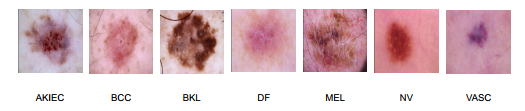
\includegraphics[width=1\linewidth]{Definitions/DataDistribution}
	\caption{Example image of each class}
	\label{fig:data-sample}
\end{figure}

More than 50 percent of lesions are confirmed through histopathology (HISTO), the ground truth for the rest of the cases is either follow-up examination (FOLLOWUP), expert consensus (CONSENSUS), or confirmation by in-vivo confocal microscopy (CONFOCAL). On the other hand, before being used for training the whole data is shuffled then split into two part. $90$ percent and $10$ percent of the data is used for training and validating respectively. Images in this data set has the type of $RGB$ and shape of (450, 600). However, Each backbone need the different input size of image as well as the range of pixel value.

\subsubsection{Metadata}
The HAM10000 data set \cite{10417} also contain the metadata of patient including gender, age, and the capturing position illustrated in Table \ref{table:metadata sample}
\begin{table}[H]
	\centering
	\begin{tabular}{|c c c c |} 
		\hline
		ID & Age & Gender & Local\\ 
		\hline
		ISIC-00001 & 15 & Male & back\\
		\hline
		ISIC-00002 & 85 & Female & elbow\\
		\hline
	\end{tabular}
	\caption{Metadata example in the data set}
	\label{table:metadata sample}
\end{table}
\subsection{Methodology}
\subsubsection{Overall Architecture}
The whole architecture of the model is represented in the Figure \ref{fig:main-model}. The model takes two input including Image data and Metadata. Metadata branch, otherwise is preprocessed before feeding into a dense layer then concatenate with the output of Soft-Attention layer. 

\begin{figure}[H]
	\centering
	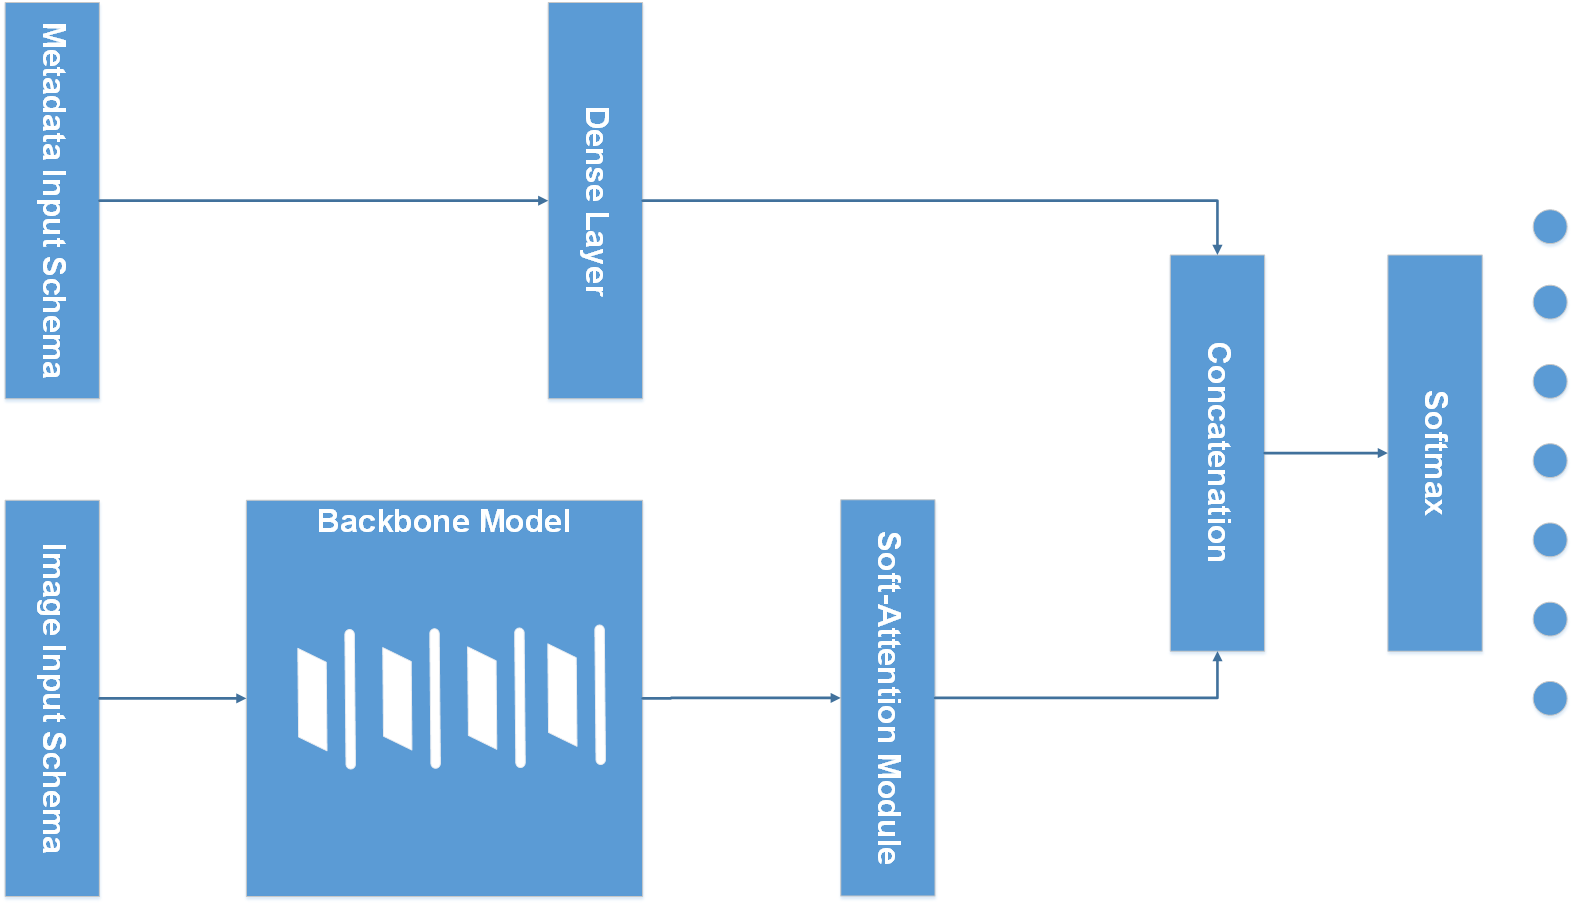
\includegraphics[width=0.8\linewidth]{Definitions/MainModel - Model Form}
	\caption{Overall Model Architecture}
	\label{fig:main-model}
\end{figure}

The Figure \ref{fig:model-structure} illustrates the overall structures of the combination of backbone models and Soft-Attention, which is used in this research. In detailed the combination of DenseNet201 and Soft-Attention is formed by replacing the three last DenseBlock, Global Average Pooling, and the fully-connected layer with the Soft-Attention Module. Similarity, ResNet50 and ResNet152 is also replaced the three last Residual Block, Global Average Pooling, and the fully connected layer with the Soft-Attention module. InceptionResNetV2, on the other hand, is replaced the Average Pool and the last Dropout with the Soft-Attention Module. Besides, the two last Normal Cell in NasNetLarge is replaced with the Soft-Attention module. 

\begin{figure}[H]
	\centering
	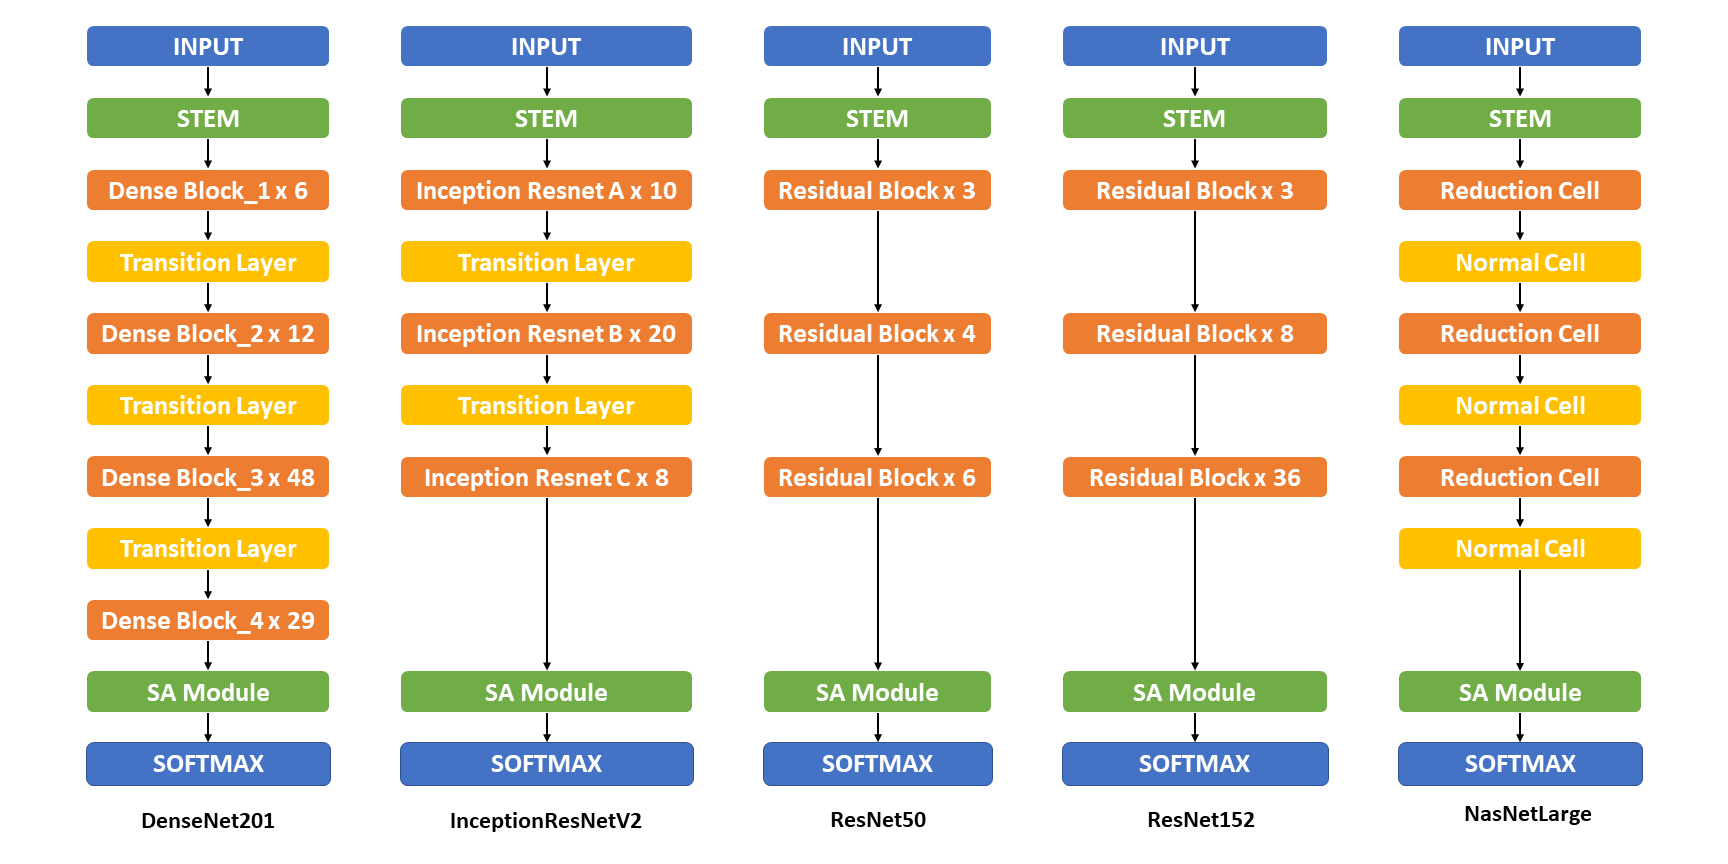
\includegraphics[width=1\linewidth]{Definitions/Model Structure}
	\caption{Overall Original Model Architecture. This figure show the overall structure of the backbone model (non mobile-based model) including DenseNet201, InceptionResNetV2, ResNet50, ResNet152, and NasNetLarge. The detail structure and information can be found at the Apendix \ref{appendix-table:detailed structure model}}
	\label{fig:model-structure}
\end{figure}

The Figure \ref{fig:mobile-model-structure}, on the other hand shows the detailed structure of mobile-based mobile and its combination with Soft-Attention. All of the MobileNet versions combine with the Soft-Attention module by replacing the two last convolution 1x1 by Soft-Attention module. The NasNetMobile, otherwise, combine with the Soft-Attention module by replacing the last Normal Cell. 
\begin{figure}[H]
	\centering
	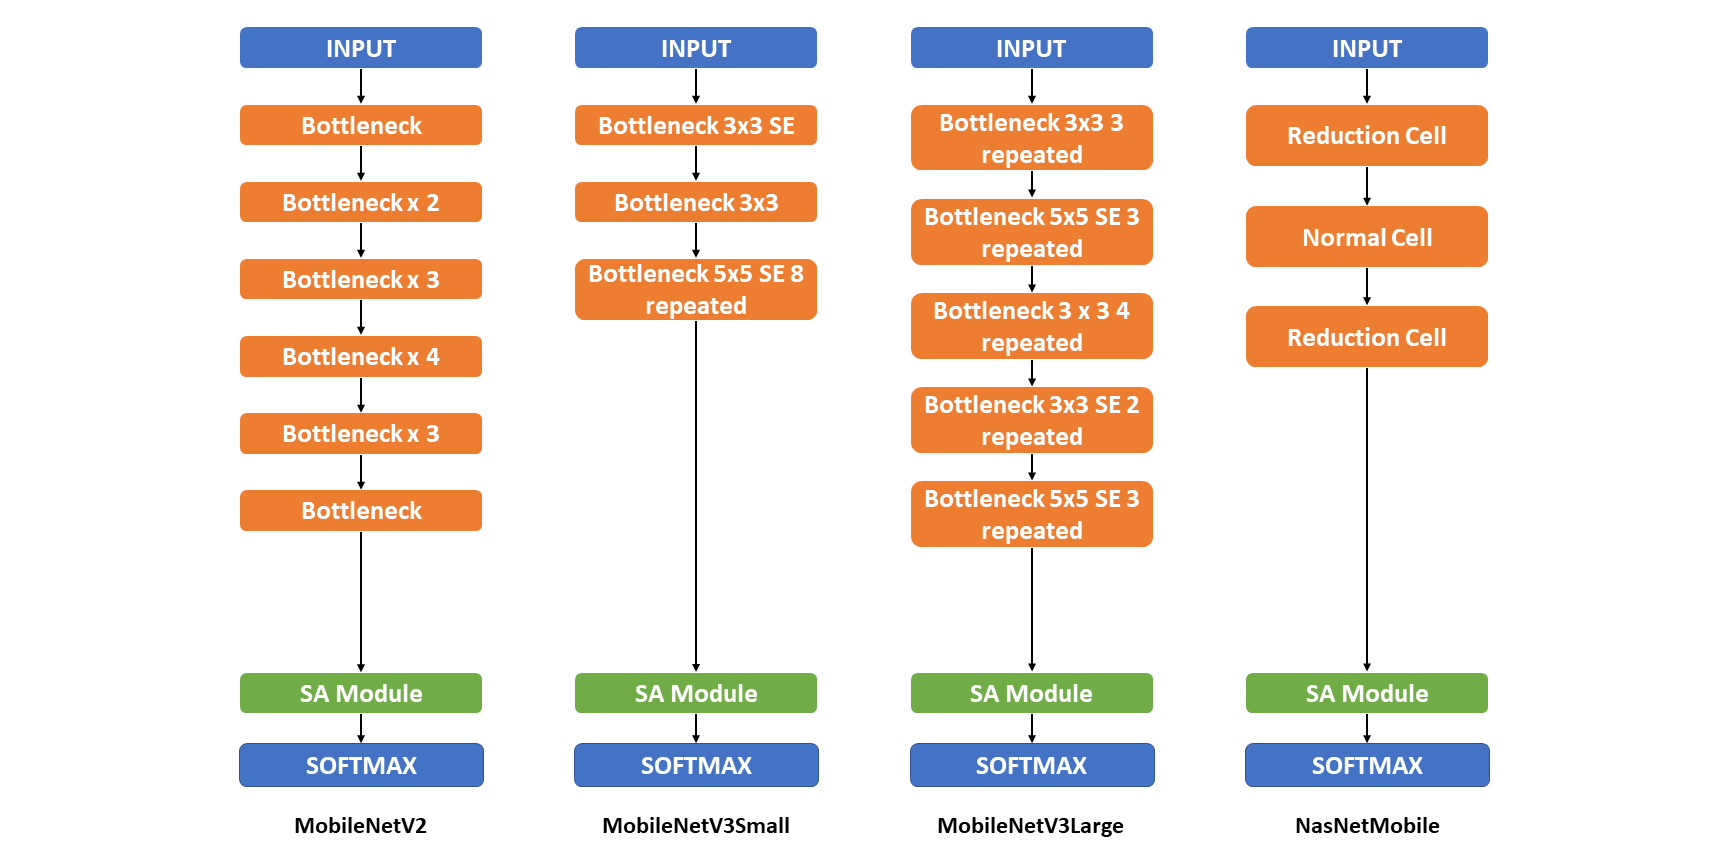
\includegraphics[width=1\linewidth]{Definitions/Mobile Model Structure}
	\caption{Overall Mobile-based Model Architecture. This figure show the overall structure of the mobile-based backbone model including MobileNetV2, MobileNetV3Small, MobileNetV3Large, and NasNetMobile. The detail structure and information can be found at the Apendix \ref{appendix-table:detailed mobile model structure}}
	\label{fig:mobile-model-structure}
\end{figure}

\subsubsection{Input Schema}
\add[H.K.D]{Image preprocessing is an essential part before the training process because of the ability to extract main pattern of an image. In this stage, the image can be changed the color channel so that the main feature is separated from the useless part. Image Retrieval, otherwise has significantly create a vector that represent the main feature of an image. Those image retrieval techniques can be energy compaction, primitive pattern units, etc. Shervan Fekri-Ershad et al create an feature vector by calculating the element wise product of histogram vector in each channel of an image \mbox{\cite{2012.4305}}. Then comparing the Euclidean distance between this feature vector and the average feature vector of the whole data set with a thresh hold, they can extract the skin part of the image.} 

In this research, the image data is both augmented for all class, the number of image increase to 18015 images and keep original form. Before feeding into the backbone model, the images is pre-processed by the input requirement of each model. DenseNet201 \cite{06993} require the input pixels values are scaled between $0$ and $1$ and each channel is normalized with respect to the ImageNet data set. In Resnet50 and Resnet152 \cite{03385} \cite{05027}, the images are converted from $RGB$ to $BGR$, then each color channel is zero-centered with respect to the ImageNet data set, without scaling. InceptionResNetV2\cite{11946}, on the other hand, will scale input pixels between $-1$ and $1$. Similarly, three versions of MobileNet \cite{04861} \cite{04381} \cite{02244}, NasNetMobile and NasNetLarge \cite{07012} require the input pixel is in range of $-1$ and $1$. 

On the other hand, the metadata is also used as another input. In the research \cite{03910}, they decide to keep the missing value and set its value to $0$. The sex and anatomical site are categorical encoded. The age, on the other hand is numerical normalized. After processing, the metadata is fed into a two-layer neural network with 256 neurons each. Each layer contains batch normalization, a ReLU \cite{08375} activation, and dropout with $p = 0.4$. The network’s output is concatenated with the CNN’s feature vector after global average pooling. Especially, they use a simply data augmentation strategy to address the problem of missing values in metadata. During training, they randomly encode each property as missing with a probability of $p = 0.1$. 

In this research, the unknowns is kept as a type as discussed in Metadata section. Sex, anatomical site and age are also category encoded and numerical normalized, respectively. After processing, the metadata is then concatenated and fed into a dense layer of 4096 neurons. Finally, this this dense layer is then concatenate with the output of Soft-Attention which is then discussed in Soft-Attention section. The Input schema is described in the Table \ref{fig:input-schema}

\begin{figure}[H]
	\centering
	\includegraphics[width=1\linewidth]{"Definitions/Input Schema"}
	\caption{Input Schema}
	\label{fig:input-schema}
\end{figure}

\subsubsection{Backbone Model}
In this paper, the backbone models used in this paper are DenseNet201 \cite{06993}, Inception \cite{00567}, MobileNets \cite{04861} \cite{04381} \cite{02244}, ResNet \cite{03385} \cite{05027}, and NasNet \cite{07012}. The combination of DenseNet201, InceptionResNetV2 and Soft-Attention layer are both tested by the previous paper \cite{03358} with a great performance. Otherwise, Resnet50 also well classify but with much less number of parameter and depth than based on its f1-score and precision stated. Therefore, in this paper, the performance of the model Resnet152 and NasnetLarge which has the larger number of parameter and depth is analyzed. On the other hand, three version of MobileNet and the NasnetMobile will also be analyzed which has a small number of parameter and depth. 

\begin{table}[H]
	\centering
	\begin{tabular}{|l | c c c|} 
		\hline
		Model & Size(MB) & Parameters & Depth \\ 
		\hline
		Resnet50 & 98 & 25.6M & 107 \\ 
		\hline
		Resnet152 & 232 & 60.4M & 311 \\ 
		\hline
		DenseNet201 & 80 & 20.2M & 402 \\
		\hline
		InceptionResNetV2 & 215 & 55.9M & 449 \\
		\hline
		MobileNet & 16 & 4.3M & 55 \\ 
		\hline
		MobileNetV2 & 14 & 3.5M & 105 \\ 
		\hline
		MobileNetV3Small & Unknown & 2.5M & 88 \\ 
		\hline
		MobileNetV3Large & Unknown & 5.5M & 118 \\
		\hline
		NasnetMobile & 23 & 5.3M & 308 \\
		\hline
		NasnetLarge & 343 & 88.9M & 533 \\ 
		\hline
	\end{tabular}
	\caption{Size and Parameters and Depth of backbone model used in this paper.}
	\label{table:model-summary}
\end{table}

\subsubsection{Soft-Attention Module}
Soft-Attention has been used in various applications: image caption generation such as \cite{03044} or handwriting verification \cite{202017}. Soft-Attention can ignore irrelevant areas of the image by multiplying the corresponding feature maps with low weights. Soft-Attention is described in the Equation \ref{eqn:softatt}.
\begin{equation}
	\label{eqn:softatt}
	f_{sa} = \gamma t\sum_{k=1}^{K}softmax(W_k * t)
\end{equation}

The Figure \ref{fig:soft-attention} shows the two main steps of applying Soft-Attention is applied in two main steps. Firstly, the input tensor is put in grid-based feature extraction from the high-resolution image, where each grid cell is analyzed in the whole slide to generate a feature map \cite{08513}. This feature map called $t \in R^{h \times w \times d}$ where $h, w, \text{and } d$ is the shape of tensor generated by a Convolution Neural Network (CNN), is then input to a 3D convolution layer whose weights is $W_k \in R^{h \times w \times d \times K}$. The output of this convolution is normalized using the soft-max function to generate K (a constant value) attention maps. These $K$ attention maps are aggregated to produce a weight function called $\alpha$. This $\alpha$ function is then multiplied with feature tensor $t$ and scaled by $\gamma$, a learnable scalar. Finally, the output of Soft-Attention function $f_{sa}$ is the concatenation of the beginning feature tensor $t$ and the scaled attention maps. 

\begin{figure}[H]
	\centering
	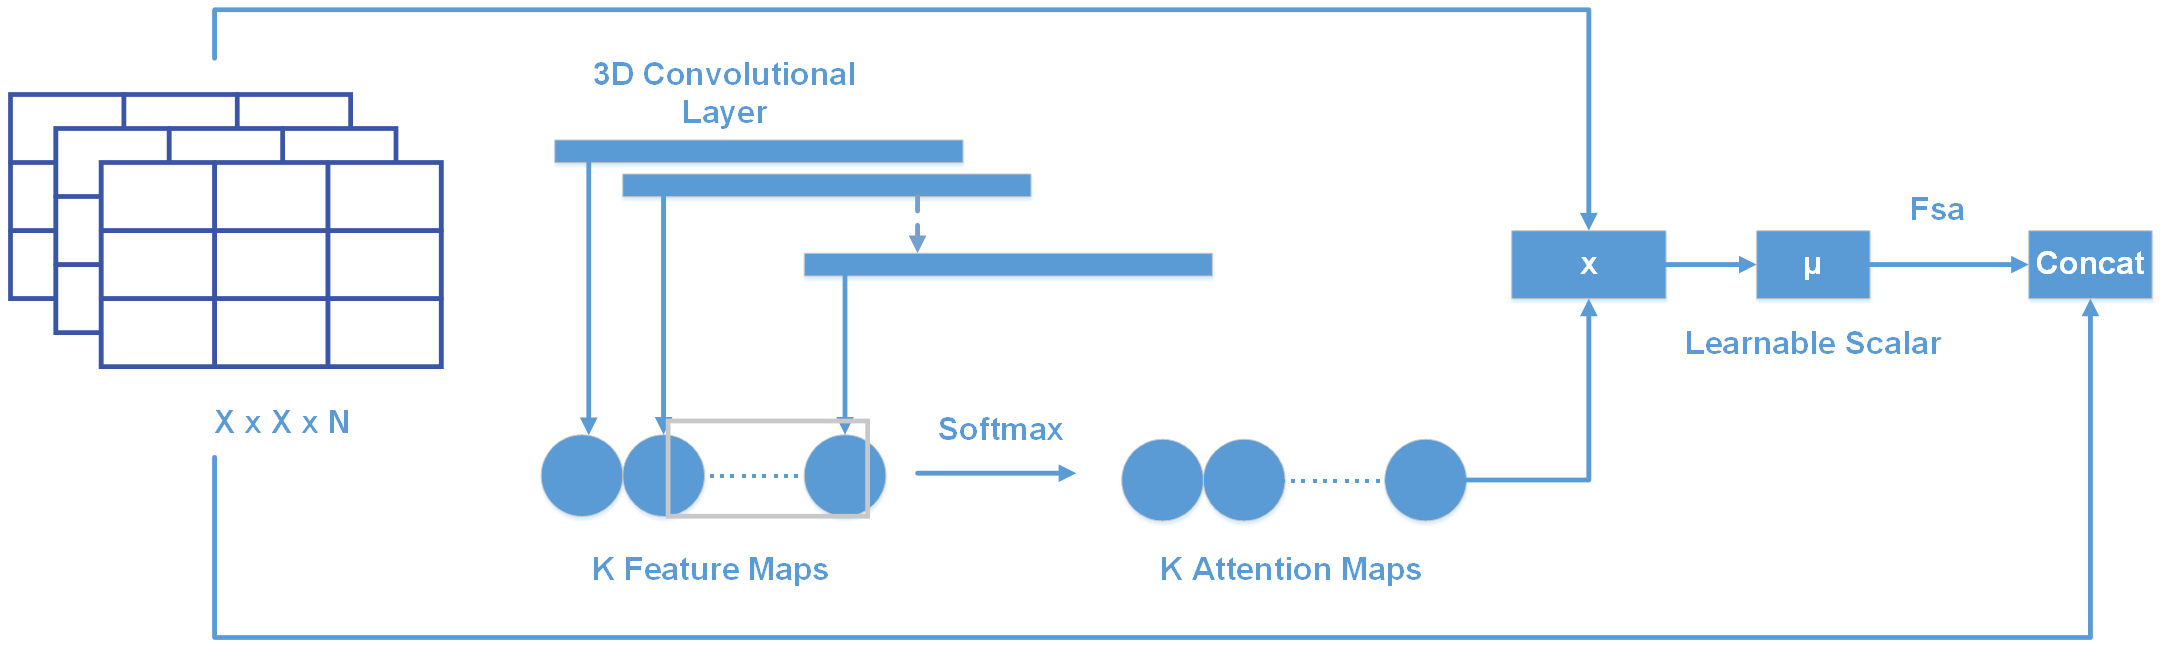
\includegraphics[width=1\linewidth]{Definitions/SoftAttention}
	\caption{Soft-Attention Layer}
	\label{fig:soft-attention}
\end{figure}

In this research, the Soft-Attention layer is applied in the same way in this research \cite{03358}. The Soft-Attention module is described in the figure \ref{fig:soft-attention-block}.

\begin{figure}[H]
	\centering
	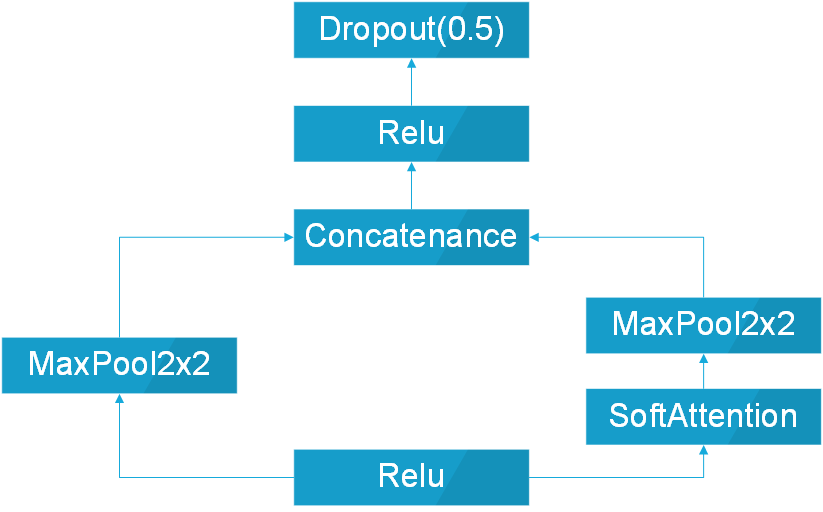
\includegraphics[width=0.5\linewidth]{Definitions/SoftAttentionBlock}
	\caption{Soft-Attention Module}
	\label{fig:soft-attention-block}
\end{figure}

After feeding into ReLU function layer, the heat feature map is processed in two paths. The first path is the 2-dimensional Max Pooling. In the second path, the feature map, on the other hand is fed into the Soft-Attention Layer before the 2-dimensional Max Pooling. After all, these two paths are then concatenated, fed into a ReLU layer, and a Dropout with the probability of $0.5$.


\subsubsection{Loss Function}
The loss function used in this paper is categorical cross-entropy. Consider $X = [x_1, x_2, \dots, x_n]$ as the input feature, $\theta = [\theta_1, \theta_2, \dots, \theta_n]$. Let $N$, and $C$ is the number of training examples and number of class respectively. The categorical cross-entropy loss is presented in the Equation \ref{eqn:weightlossfunction}.
\begin{equation}
	\label{eqn:weightlossfunction}
	L(\theta, x_n) = -\frac{1}{N}\sum_{c=1}^{C}\sum_{n=1}^{N}W_c\times y^c_n \times \log(\hat{y}^c_n)
\end{equation}

where $\hat{y}^c_i$  is the output of model and $y^c_i$ is the target that the model should return, $W_c$ is the weight of class $c$. Since the data set face the imbalanced problem then class weight for the loss is applied. In this research, both of the original weight and a new weight formula is implementation. Originally, the weight is calculated by taking the inverse of percentage that each class accounts for. The new weight formula is described in the Equation \ref{eqn:weightformula} and \ref{eqn:vector-inverse-percent}. \add{This weight formula is the original weight multiplies with the inverse of number of class in the data set which make the training more balanced. It is inspired by the “balanced” heuristic proposed by Gary King et al\mbox{\cite{WV006-01}}}

\begin{equation}
	\label{eqn:weightformula}
	W = N \odot D
\end{equation}

\begin{equation}
	\label{eqn:vector-inverse-percent}
	D = \begin{bmatrix}
		\frac{1}{C \times  N_1} & \frac{1}{C \times  N_2} & \dots & \frac{1}{C \times  N_n}\\
	\end{bmatrix} = \frac{1}{C} \odot \begin{bmatrix}
		\frac{1}{N_1} & \frac{1}{N_2} & \dots & \frac{1}{N_n}\\
	\end{bmatrix}
\end{equation}

where $N$ is the number of training sample, $C$ is the number of class, $N_i$ is the number of sample in each class $i$. $D$ is the matrix contain the inverse of $C \times N_i$. 

%%%%%%%%%%%%%%%%%%%%%%%%%%%%%%%%%%%%%%%%%%
\section{Results}
\subsection{Experimental Setup}
\subsubsection{Training}
Before training, the data set is split into two sub set for training (90 percent) and validation (10 percent). Test set, otherwise is provided by the HAM10000 data set, contains 857 images. To analyze the effect of augmented data on the model, before the training the image data is augmented to $53573$ images by the following technique:\\
- Rotation Range: rotate the image in an \add[H.K.D]{angle range of 180}. \\
- Width and height shift range: Shift the image horizontally and vertically \add[H.K.D]{in a range of 0.1}, respectively. \\
- Zoom Range:  Zoom in or zoom out the image \add[H.K.D]{in a range of 0.1} to create new image. \\
- Horizontal and vertical flipping: Flipping the image horizontally and vertically to create new image.\\
Otherwise, all of models is trained with the Adam Optimizer \cite{6980} with the learning rate of $0.001$ which is reduced by a factor of $0.2$ to a minimum learning rate of $0.1 x 10^6$, and the epsilon is set to $0.1$. The initial epochs is set to 250 epochs and the Early Stopping is also applied to stop the training as the accuracy of validation set does not increase after $25$ epochs. Besides, the batch size is set to $32$.

\subsubsection{Tools}
TensorFlow and Keras are two of the most popular framework to build deep learning model. In this research, Keras based on TensorFlow is used to build, clone the backbone model which is pre-trained with the image-net data set. Otherwise, the models are trained by NVIDIA RTX TitanV and the data set is pre-processed with the CPU Intel I5 32 processors, RAM 32GB. In detail, the GPU is setup with CUDA 11.6, cuDNN 8.3 and ChipSRT as the requirement of TensorFlow version 2.7.0.
\subsubsection{Evaluation Metrics}
\begin{figure}[!htb]
	\begin{minipage}{0.48\textwidth}
		\centering
		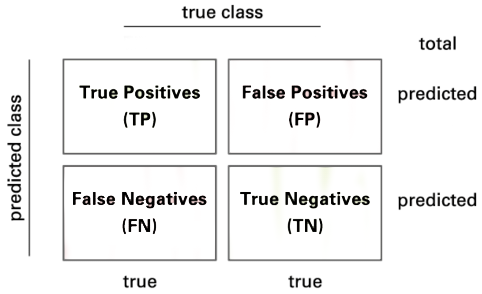
\includegraphics[width=1.1\linewidth]{Definitions/Confusion-matrix}
		\caption{Confusion Matrix}\label{fig:confusion-matrix}
	\end{minipage}\hfill
	\begin{minipage}{0.48\textwidth}
		\centering
		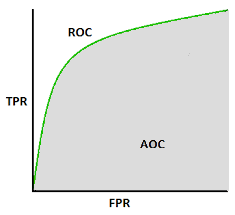
\includegraphics[width=.7\linewidth]{Definitions/AUC}
		\caption{Area Under the Curve}\label{fig:AUC}
	\end{minipage}
\end{figure}
The model is evaluated by using the confusion matrix and related metrics. The Figure \ref{fig:confusion-matrix} illustrates the presentation of a $2 \times 2$ confusion matrix used for $2$ class. Consider a confusion matrix $A$ with $C$ number of class. Let $A^i$ and $A^j$ is the set of $A$ rows and columns respectively, therefore $A^i_k$ is the element at row i and column k
\[
A = \begin{bmatrix}
	a_{11} & a_{12} & \dots & a_{1j} \\
	a_{21} & a_{22} & \dots & a_{2j} \\
	\vdots & \vdots	&  & \vdots\\
	a_{i1} & a_{i2} & \dots & a_{ij} 
\end{bmatrix}
\]
The True Positive(TP) of all class in this case is the main diagonal of the matrix $A$. The following method are used to calculate the False Positives(FP), False Negatives(FN), and True Negatives(TN) of all class:

\begin{equation}
	\label{eqn:FP}
	FP = -TP + \sum_{k=1}^{i}A^i_k
\end{equation}

\begin{equation}
	\label{eqn:FN}
	FN = -TP + \sum_{k=1}^{j}A^j_k
\end{equation}

\begin{equation}
	\label{eqn:TN}
	TN_c = \sum_{i=1}^{C}\sum_{j=1}^{C}a_{ij} - \left[ \sum_{k=1}^{i}A^i_{i=c k} + \sum_{k=1}^{j}A^j_{j=c k} \right] + a_{i=c j=c} \implies TN = \begin{bmatrix}
		TN_1 & TN_2 & \dots & TN_c
	\end{bmatrix}
\end{equation}

Then, the model is evaluated by the following metrics:

\begin{equation}
	\label{eqn:sens}
	\text{Sensitivity (Sens)} = \frac{TP}{TP + FN}
\end{equation}

\begin{equation}
	\label{eqn:spec}
	\text{Specificity (Spec)} = \frac{TN}{TN + FP}
\end{equation}

\change[H.K.D]{Sensitivity  and Specificity  mathematically describe the accuracy of a test which reports the presence or absence of a condition. Individuals for which the condition is satisfied are considered "positive" and those for which it is not are considered "negative". Sensitivity or true positive rate refers to the probability of a positive test, conditioned on truly being positive while Specificity  or true negative rate refers to the probability of a negative test, conditioned on truly being negative.}{Sensitivity (Equation \mbox{\ref{eqn:sens}}) and Specificity (Equation \mbox{\ref{eqn:spec}}) mathematically describe the accuracy of a test that identifies a condition's presence or absence. Sensitivity, also known as the true positive rate, is the likelihood that a test will result in a true positive, whereas specificity, also known as the true negative rate, is the likelihood that a test will result in a true negative.}

\begin{equation}
	\label{eqn:pre}
	\text{Precision} = \frac{TP}{TP + FP}
\end{equation}
	
\begin{equation}
	\label{eqn:f1}
	\text{F1 Score} = \frac{2 \times TP}{2 \times TP + FP + FN + TN}\
\end{equation}

Precision (Equation \ref{eqn:pre}) or positive predictive value (PPV) is the probability of a positive test conditioned on both truly being positive or negative. F1-score (Equation \ref{eqn:f1}), on the other hand refers the harmonic mean of precision and recall which mean the higher the f1-score is, the higher both precision and recall is. Besides, the expected value of precision, f1-score and recall-score are also applied because of the multi-class problem.

\begin{equation}
	\label{eqn:acc}
	\text{Accuracy} = \frac{TP + TN}{TP + FP + FN + TN}
\end{equation}

\begin{equation}
	\label{eqn:balacc}
	\text{Balanced Accuracy} = \frac{\text{Sens} + \text{Spec}}{2}
\end{equation}

The last metric is the $AUC$ score standing for Area Under the Curve which is the Receiver Operating Curve (ROC) that indicate the probability of TP versus the probability of FP.  

\subsection{Discussion} 
\begin{comment}
	\begin{figure}[H]
		\centering
		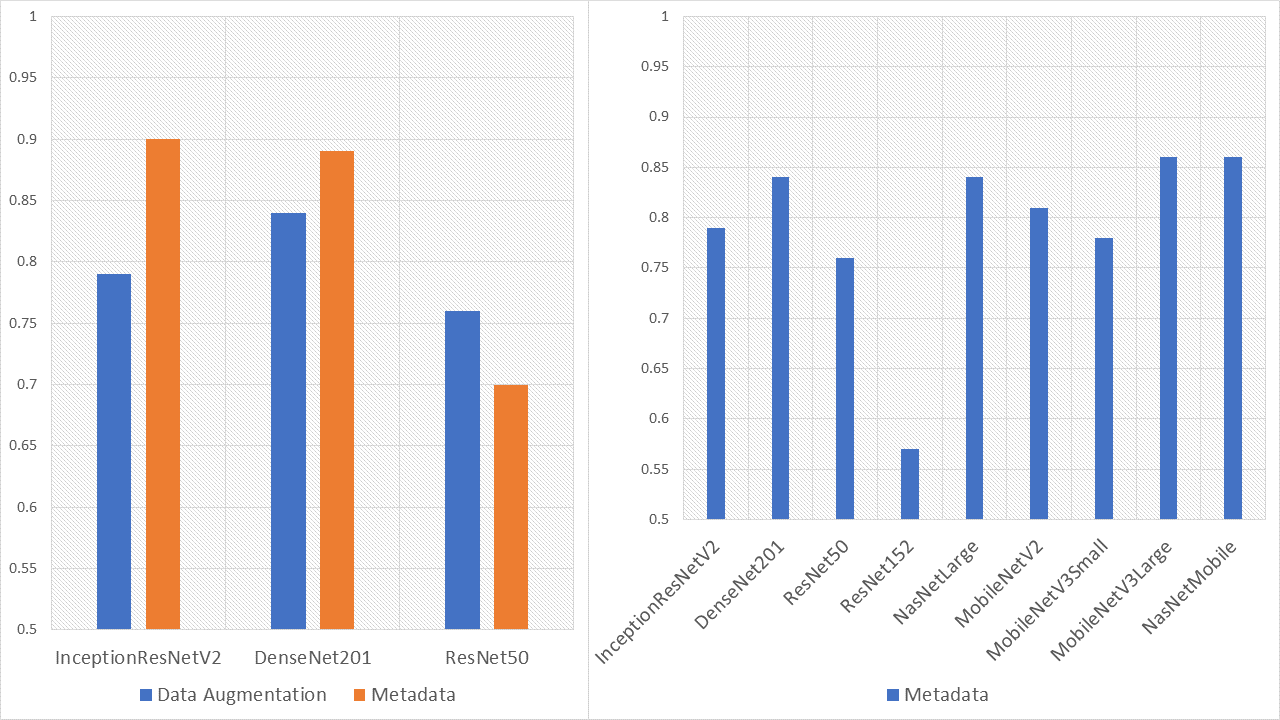
\includegraphics[width=1\linewidth]{Definitions/ACCALL}
		\caption{Accuracy of all models trained in this research}
		\label{fig:accall}
	\end{figure}
\end{comment}

According to the Table \ref{table:overall-acc}, it is clear that the model trained with metadata has a higher accuracy than the model trained with augmented data only. While InceptionResNetV2 and DenseNet201 trained with augmented data have accuracy of $0.79$ and $0.84$ respectively, their training with metadata are $0.90$ and $0.89$, respectively. Furthermore, Resnet50 trained with metadata data has the accuracy that outperform the Resnet50 trained with augmented data and is twice as high as Resnet152 trained with metadata. On the other hand, mobile model including MobileNetV2, MobileNetV3Large, and NasNetMobile, even though has a much smaller number of parameters and depth than the other model, they have a quite good accuracy of $0.81$, $0.86$, $0.86$, respectively. 

\begin{table}[H]
	\centering
	\begin{tabular}{| l | c  c | }
		\hline
		Model & ACC(AD) & ACC(MD)\\ 
		\hline
		InceptionResNetV2 & 0.79 & \textbf{0.90}\\
		\hline
		DenseNet201 & 0.84 & \textbf{0.89}\\
		\hline
		ResNet50 & 0.76 & 0.70\\
		\hline
		ResNet152 & 0.81 & 0.57\\
		\hline
		NasNetLarge & - & 0.84\\
		\hline
		MobileNetV2 & 0.83 & 0.81\\
		\hline
		MobileNetV3Small & - & 0.78\\
		\hline
		MobileNetV3Large & 0.85 & \textbf{0.86}\\
		\hline
		NasNetMobile & 0.84 & \textbf{0.86}\\
		\hline
	\end{tabular}
	\caption{Accuracy of all models. ACC stands for accuracy. AD stands for augmented data, this indicate that the model is trained with augmented data. MD stands for Metadata which indicate that the model is trained with Metadata}
	\label{table:overall-acc}
\end{table}

Moreover, the model trained with augmented data does not only have low accuracy but their f1-score and the recall score also are imbalanced according to Figure \ref{fig:den f1}, \ref{fig:incep f1}, \ref{fig:den recall}, and \ref{fig:incep recall}. As a results, augmented data model does not classify well on all class as InceptionResNetV2 trained on augmented data have f1-score on class df and akiec is just above $0.3$ and $0.4$, separately while InceptionResNetV2 trained on metadata and the new weight loss can classify well in a balanced way arcoding to the Figure \ref{fig:incep f1}. However, only DenseNet201, InceptionResNetV2, and NasNetLarge whose depth are equal or larger than 400 have balanced f1-score on class. The others still face the imbalanced term. Since this data set is not balanced, therefore using augmented data can make the model more  bias to the class which has larger sample. Using the metadata, though still make the model bias, it does contributes to the improvement of  the performance of the model.

\begin{figure}[!htb]
	\begin{minipage}{0.48\textwidth}
		\centering
		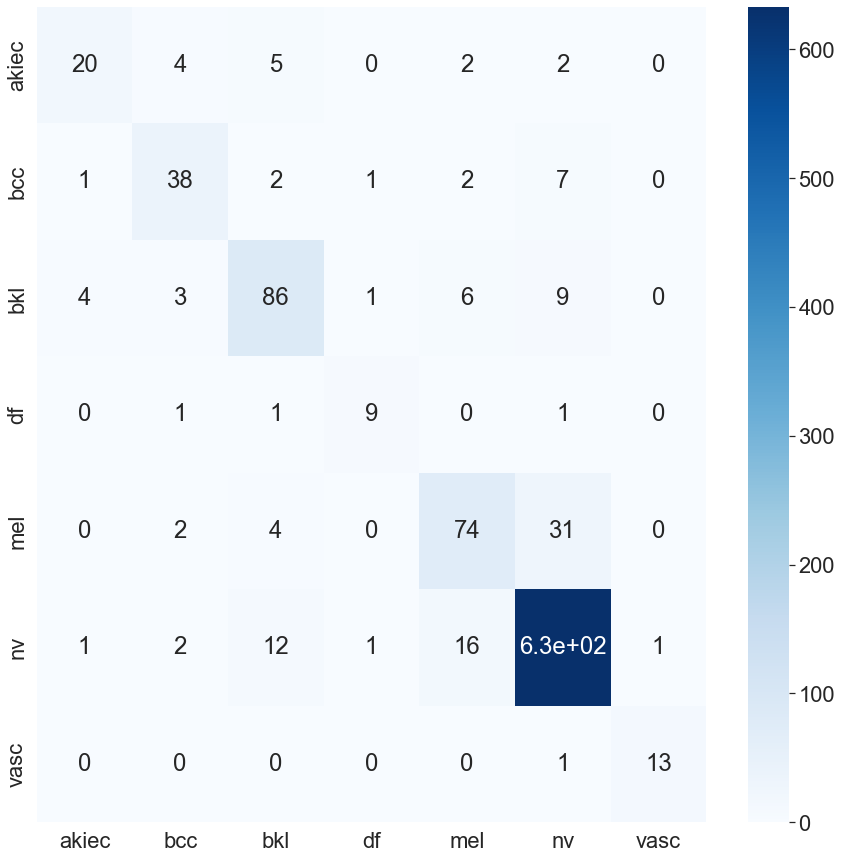
\includegraphics[width=1\linewidth]{Definitions/CM/dn201cm}
		\caption{DenseNet201 Confusion Matrix}\label{fig:densenet201cm}
	\end{minipage}\hfill
	\begin{minipage}{0.48\textwidth}
		\centering
		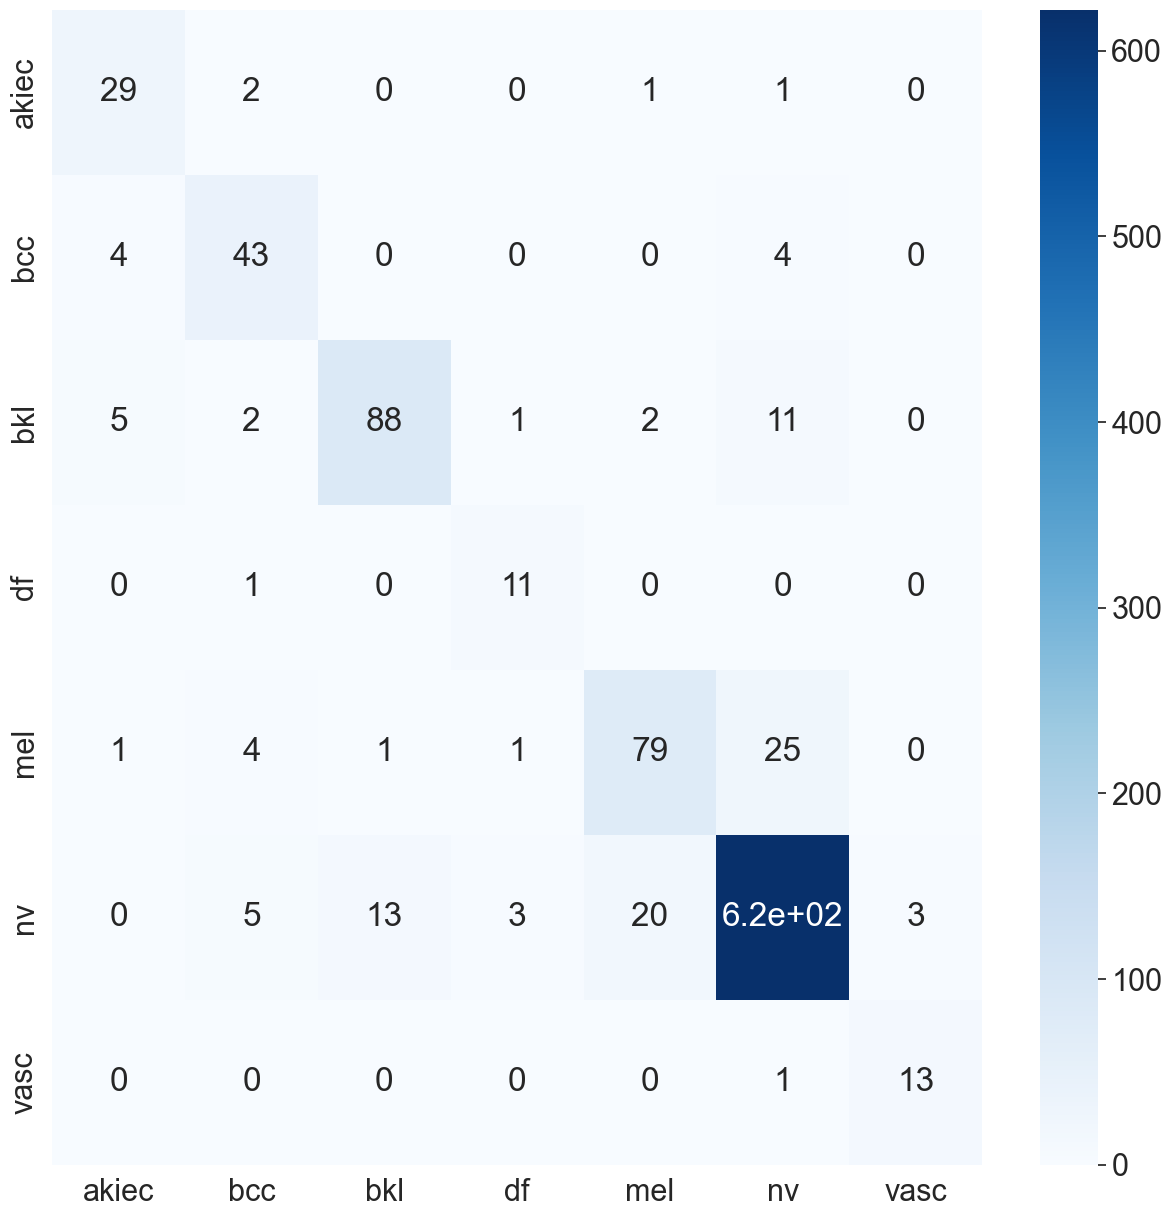
\includegraphics[width=1\linewidth]{Definitions/CM/irv2cm}
		\caption{InceptionResNetV2 Confusion Matrix}\label{fig:irv2cm}
	\end{minipage}
\end{figure}

\begin{figure}[H]
	\centering
	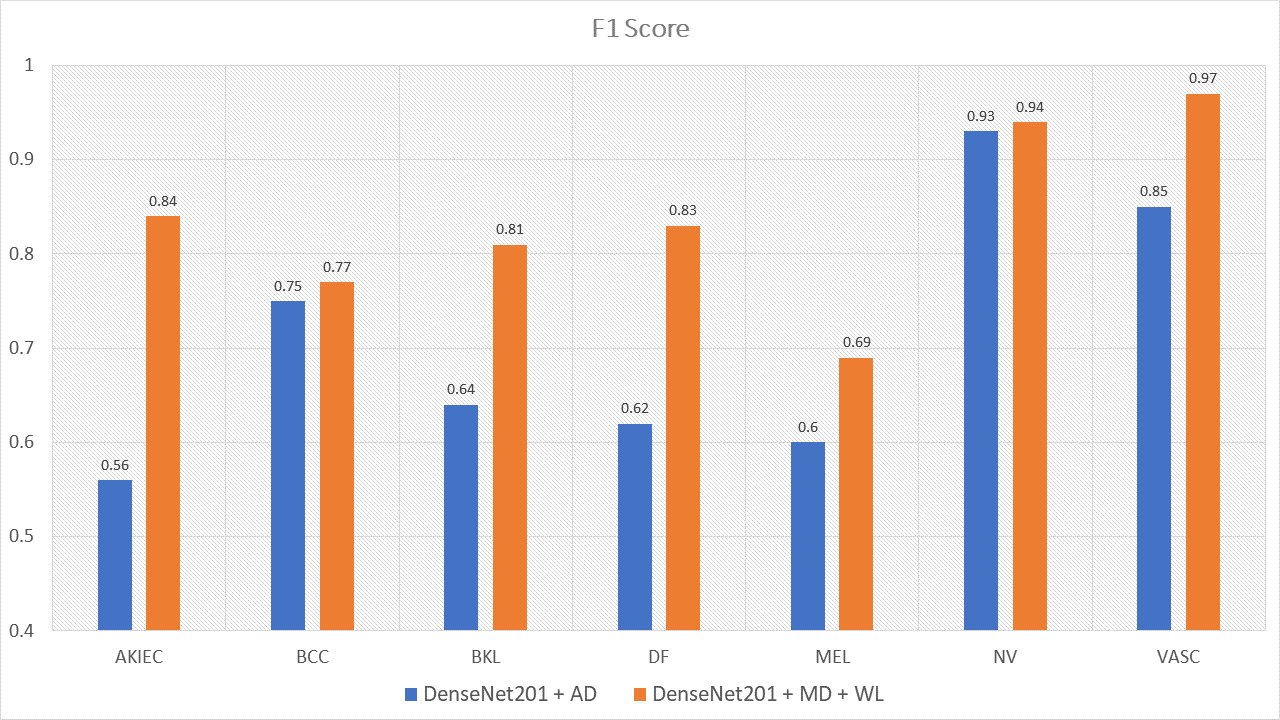
\includegraphics[width=1\linewidth]{Definitions/den f1}
	\caption{The comparison between f1 scores of DenseNet201 trained with augmented data and the one trained with metadata and weight loss}
	\label{fig:den f1}
\end{figure}
\begin{figure}[H]
	\centering
	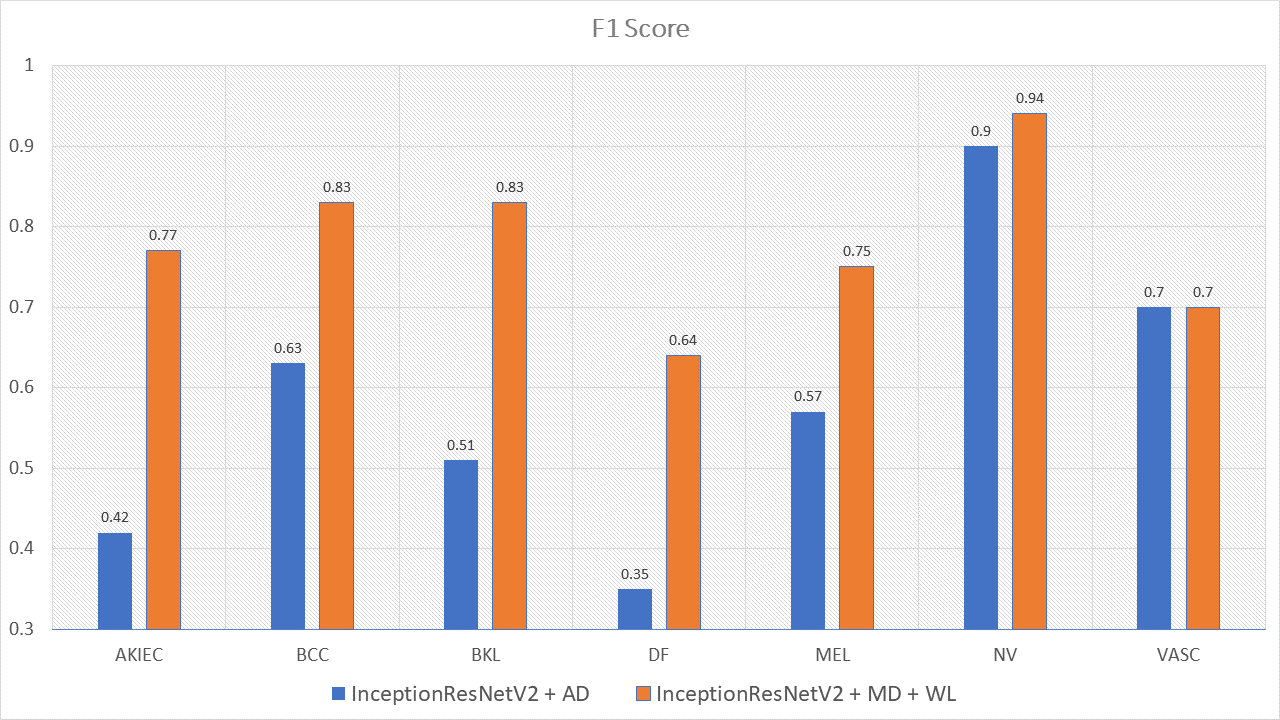
\includegraphics[width=1\linewidth]{Definitions/in f1}
	\caption{The comparison between f1 scores of InceptionResNetV2 trained with augmented data and the one trained with metadata and weight loss}
	\label{fig:incep f1}
\end{figure}

This problem is also true with the recall score according to Figure \ref{fig:den recall} and \ref{fig:incep recall}. DenseNet201, InceptionResNetV2, trained with augmented data has expected value of recall of $0.56$, $0.69$, respectively, while the combination of DenseNet201, Metadata and the new weight loss function achieve the expected value of recall: $0.82$. Therefore, metadata does improve the model performance by reducing the amount of data needed for achieving higher results. On the other hand, the reason why the model become much more balanced is the weighted loss function. Weight loss function has ability to solve the imbalanced class samples by adding a weight related to the number of samples in each class. DenseNet201, InceptionResNetV2 trained with the new weighted loss function have recall in akiec of $0.85$. $0.82$, respectively, as opposed to their training in akiec without weighted loss function: $0.65$ and $0.37$. 

\begin{figure}[H]
	\centering
	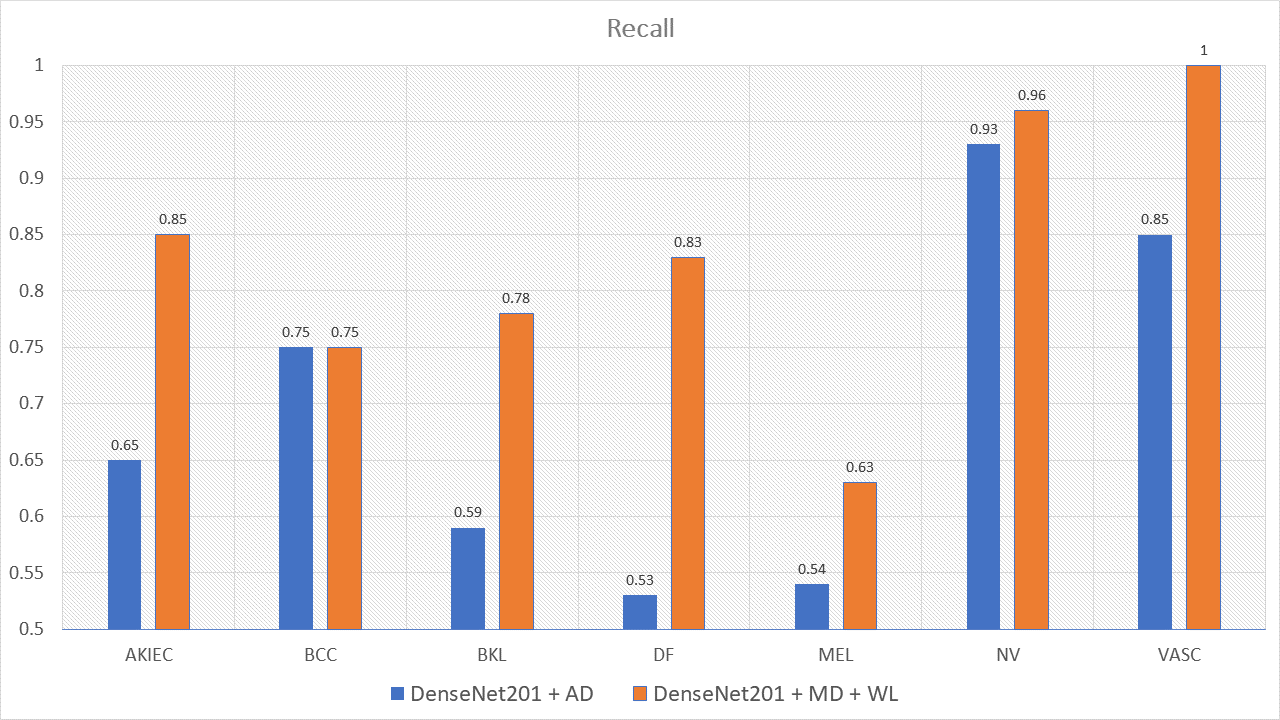
\includegraphics[width=1\linewidth]{Definitions/den re}
	\caption{The comparison between recal scores of DenseNet201 trained with augmented data and the one trained with metadata and weight loss}
	\label{fig:den recall}
\end{figure}

\begin{figure}[H]
	\centering
	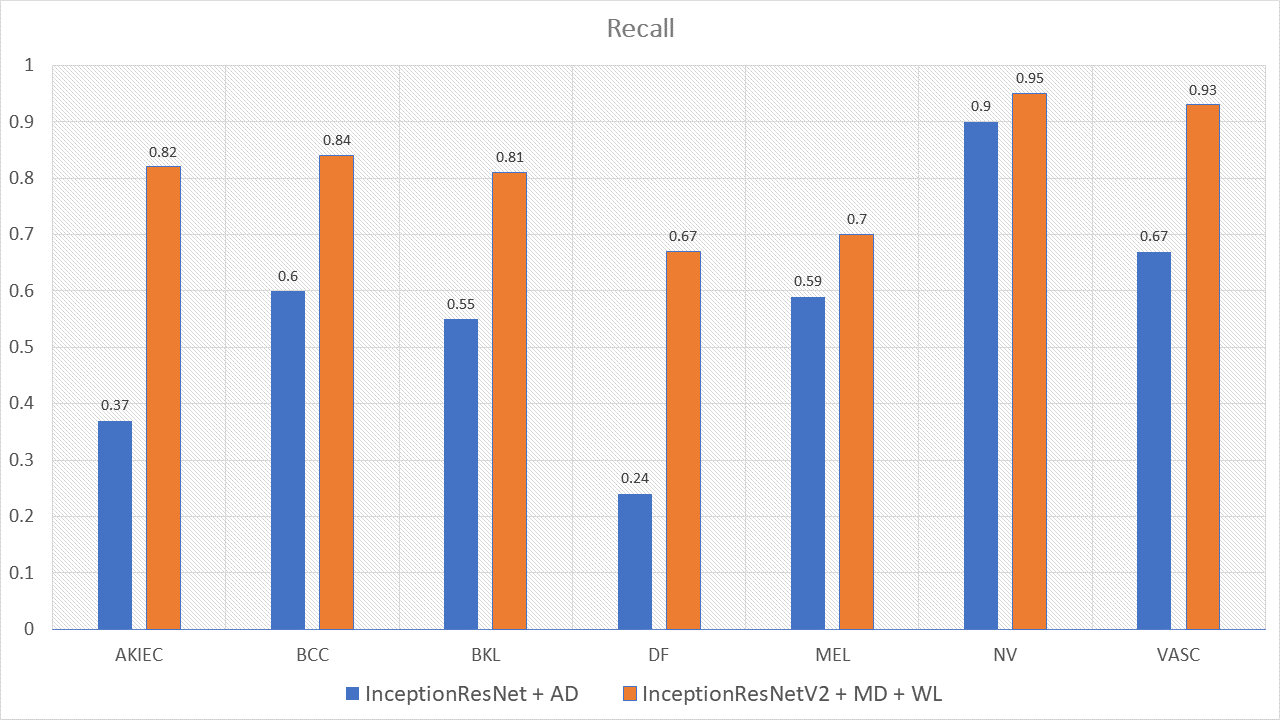
\includegraphics[width=1\linewidth]{Definitions/in re}
	\caption{The comparison between recall scores of InceptionResNetV2 trained with augmented data and the one trained with metadata and weight loss}
	\label{fig:incep recall}
\end{figure}

Another interesting point found during the experiment is that MobileNetV2, MobileNetV3 and NasNetMobile have small number of parameters and depth, though have relative good performance. MobileV3large, MobileV3Small, NasNetLarge and NasNetMobile outperform others on classifying class df with the recall score of $0.92$, $1$, $0.92$, $0.92$, separately according to the Table \ref{appendix-table:mobile-performance}. It's transparent that MobileNetV3Large and NasNetMobile are the two best performance model. Nevertheless, MobileNetV3Large has less number of parameters and depth than NasNetMobile.

\begin{table}[H]
	\centering
	\begin{tabular}{| l | c | c | c |}
		\hline
		Model & MobileNetV3Large & DenseNet201 & InceptionResnetV2\\
		\hline
		No. Trainable Parameters & \textbf{5,490,039} & 17,382,935 & 47,599,671\\
		\hline
		Depth & \textbf{118} & 402 & 449\\
		\hline
		Accuracy & 0.86 & 0.89 & 0.90\\
		\hline
		Time Prediction(s/epochs) & \textbf{116} & 1000 & 3500 \\
		\hline
		Computational Complexity & & &\\		
		\hline
	\end{tabular}
	\caption{\change[H.K.D]{Performance Comparison between MobileNetV3Large and DenseNet201, InceptionResNetV2}{How Performance of MobileNetV3Large be optimized}}
	\label{table:optimized-performance-mobile-model}
\end{table}

The Table \ref{table:optimized-performance-mobile-model} shows that the MobileNetV3Large, though the number of parameters are much smaller than the DenseNet201, InceptionResNetV2, achieve the accuracy nearly to the others. In detail, MobileNetV3Large whose the number of parameters is 5.5 millions which is four and ten times less than DenseNet201 and InceptionResNetV2, respectively. The depth of MobileNetV3Large, on the other hand, is four times less than DenseNet201, InceptionResNetV2 which are 118 hidden layers as opposed to 402, 449 of DenseNet201 and InceptionResNetV2, separately. Although, the MobileNetV3Larege only achieve the accuracy of 0.86 the time need for prediction is 10 and 30 times less than the other opponents. If the MobileNetV3Large need a harder process of parameter hyper-tuning to achieve a better result, which is also the future target of this research.

The Table \ref{table:overall-auc} shows the AUC score of the three models InceptionResNetV2, Densenet201, and ResNet50 which is trained with only augmented data or metadata. It's transparent that the InceptionResNetV2 and DenseNet201 have higher AUC-score trained with metadata: 0.974 and 0.971 as opposed to 0.972 and 0.93, respectively. ResNet50 trained with augmented data, on the other hand have higher auc-score: 0.95 as compared to 0.93 of ResNet50 trained with metadata. Overall, InceptionResNetV2 trained with metadata reach the peak with the auc-score of 0.974. The InceptionResNetV2 trained with metadata is also compared with the others to find out the best models trained. According to the figure 15, the InceptionResNetV2 still hit the peak of 0.974 auc-score. ResNet152, otherwise is the worst model with the auc-score of 0.87. Other models, on the other hand have the approximately same of auc-score. 

\begin{table}[H]
	\centering
	\begin{tabular}{| l | c  c | }
		\hline
		Model & AUC(AD) & AUC(MD)\\ 
		\hline
		InceptionResNetV2 & 0.971 & \textbf{0.99}\\
		\hline
		DenseNet201 & 0.93 & \textbf{0.99}\\
		\hline
		ResNet50 & \textbf{0.95} & 0.93 \\
		\hline
		ResNet152 & 0.97 & 0.87\\
		\hline
		NasNetLarge & - & \textbf{0.96}\\
		\hline
		MobileNetV2 & 0.95 & \textbf{0.97}\\
		\hline
		MobileNetV3Small & 0.67 & \textbf{0.96}\\
		\hline
		MobileNetV3Large & 0.96 & \textbf{0.97}\\
		\hline
		NasNetMobile & 0.96 & \textbf{0.97}\\
		\hline
	\end{tabular}
	\caption{AUC (area under the curve) of all models. AD stands for augmented data, this indicate that the model is trained with augmented data. MD stands for Metadata which indicate that the model is trained with Metadata}
	\label{table:overall-auc}
\end{table}

\begin{figure}[!htb]
	\centering
	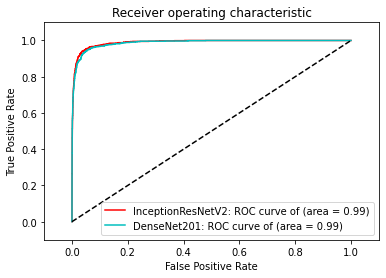
\includegraphics[width=1\linewidth]{Definitions/ROC/denvsirv2}
	\caption{ROC of DenseNet201 and InceptionResNetV2}\label{fig:densenet201auc}
\end{figure}

Besides the comparison between original weight loss calculated by the sample percentage of each class model and the new weight loss based model is also conducted on the three best performance model including InceptionResNetV2, DenseNet201, MobileNetV3. After the experiment, it is found out that the new weight loss function dose not only contribute to the model to overcome the data imbalance problem but it also make the accuracy increase. The performance of models is described in the Table \ref{table:loss-comparision}

\begin{table}[H]
	\centering
	\begin{tabular}{| l | c | c | c |}
		\hline
		Model & No Weight & Original Loss Accuracy & New Loss Accuracy\\
		\hline
		InceptionResNetV2 & 0.74 & 0.79 & 0.90\\
		DenseNet201 & 0.81 & 0.84 & 0.89\\
		MobileNetV3 & 0.79 & 0.80 & 0.86\\
		\hline
	\end{tabular}
	\caption{Loss based model accuracy comparison}
	\label{table:loss-comparision}
\end{table} 

After reviewing, the InceptionResNetV2 is found to be the best model trained. Futhermore, the InceptionResNetV2 is compared with the other state of the art researched model. According to the Table \ref{table:comparative-analysis}, there are six research that use the same data set: HAM10000 but different approaches. These models used in that research are also SOTA models sorted in ascending order. The Table shows that the accuracy of the combination of InceptionResNetV2 with Soft-Attention, metadata and weight loss in this research is less than the InceptionResNetV2 with Soft-Attention and augmented data: 0.90 compared to 0.93 respectively. However, since Soumyyak et al use data augmentation for all class of an imbalanced data set, the f1-score and recall score are much lower. This is because the model in that research can only classify well on NV and VASC class which have the highest number of samples. On the other hand, the InceptionResNetV2 in this research also outperform the other model according to 5 indicator: accuracy, precision, f1-score, recall score, and auc score. 
\FloatBarrier
\begin{table}[H]
	\centering
	\begin{tabular}{| p{4cm} | c | c | c | c | c |}
		\hline
		Model & Accuracy & Precision & f1-score & recall & auc-score\\
		\hline
		Our Proposed & 0.9	& 0.86 &\textbf{0.86} & \textbf{0.81} & \textbf{0.99}\\
		\hline
		InceptionResNetV2\cite{03358} & 0.93 & 0.89 & 0.75 & 0.71 & \textbf{0.99}\\
		\hline
		\cite{03798} & - & 0.88 & 0.77 & 0.74 & - \\
		\hline
		\cite{09418} & 0.88 & - & - & - & - \\
		\hline
		\cite{01284} & 0.86 & - & - & - & - \\
		\hline
		GradCam and Kernel SHAP\cite{06612} & 0.88 & - & - & - & - \\
		\hline
		Student and Teacher\cite{03225} & 0.85 & 0.76 & 0.76 & - & - \\
		\hline
	\end{tabular}
	\caption{Comparative Analysis}
	\label{table:comparative-analysis}
\end{table} 

However, there is still some drawbacks of the model that the InceptionResNetV2 cannot well classify the melanoma and the nevus. According to Figure \ref{fig:nevusVSmela} the model sometime classify the black nevus as the melanoma because of the same color between them. However, this problem is not true for the hard black or big melanoma or the red black nevus. Some future approach that can be proposed are change the type of color to other to fix the same color problem.

\begin{figure}[H]
	\centering
	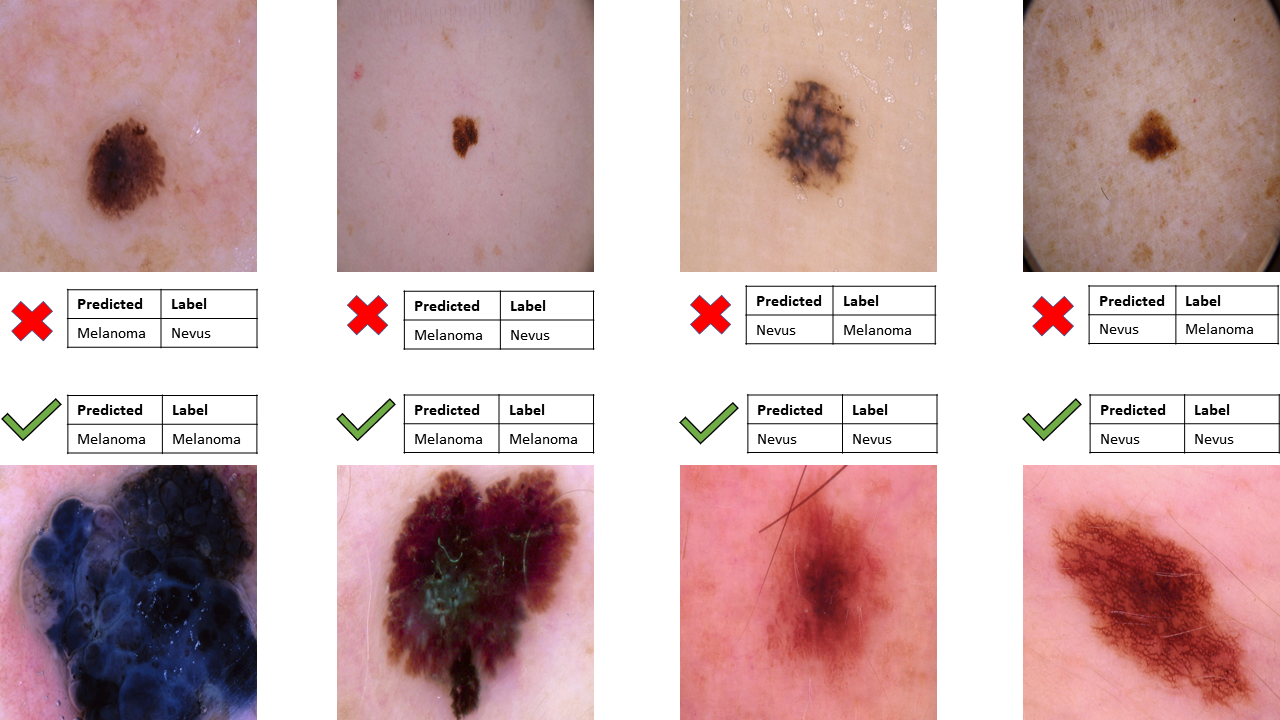
\includegraphics[width=1\linewidth]{Definitions/img_class_nevus_mela}
	\caption{Model ability to classify melanoma and nevus}
	\label{fig:nevusVSmela}
\end{figure}

\section{Conclusions}
In this research, our proposed is to construct a model as a combination of backbone models and Soft-Attention. Moreover, the model takes two inputs including image data and metadata. besides, a new weight loss function is applied to figure out the data imbalance problem. Finally, the combination of InceptionResNetV2, Soft-Attention, and Metadata is the best model with the accuracy of 0.9. Although the accuracy and the precision of the model are not the highest, the f1-score, recall, and AUC-score of 0.86, 0.81 and 0.975, respectively is the highest and the most balanced indicator. Therefore, InceptionResnetV2 can classify well in all classes including low samples classes. Otherwise, during the experiment, the combination of MobileNetV3, Soft-Attention, and Metadata achieve an accuracy of 0.86 that is nearly the same as InceptionResNetV2, though with fewer number parameters and depth. Therefore the infer time is much less than the InceptionResNetV2. This result opens the door to constructing a great performance model that can be applied to mobile, IoT devices. \add[H.K.D]{As the result, proposed method and others still face the problem of badly distinguish between melanoma and black nevus because in some cases, the melanoma and the nevus image has the same lesion size and color.}
\vspace{6pt} 

%%%%%%%%%%%%%%%%%%%%%%%%%%%%%%%%%%%%%%%%%%
%% optional
%\supplementary{The following supporting information can be downloaded at:  \linksupplementary{s1}, Figure S1: title; Table S1: title; Video S1: title.}

% Only for the journal Methods and Protocols:
% If you wish to submit a video article, please do so with any other supplementary material.
% \supplementary{The following supporting information can be downloaded at: \linksupplementary{s1}, Figure S1: title; Table S1: title; Video S1: title. A supporting video article is available at doi: link.}

%%%%%%%%%%%%%%%%%%%%%%%%%%%%%%%%%%%%%%%%%%
\authorcontributions{Conceptualization, V.D.N. and H.K.D.; methodology, V.D.N. and H.K.D.; software, K.D.; validation, V.D.N., N.D.B. and H.K.D.; formal analysis, V.D.N. and H.K.D.; investigation, V.D.N., N.D.B. and H.K.D.; resources, V.D.N.; data curation, H.K.D.; writing---original draft preparation, H.K.D.; writing---review and editing, V.D.N. and N.D.B.; visualization, H.K.D.; supervision, V.D.N. and N.D.B.; project administration, V.D.N. All authors have read and agreed to the published version of the manuscript.}

\funding{This research received no external funding}

\institutionalreview{Not applicable}

\informedconsent{Not applicable}

\dataavailability{The code and the data analysis report can be found here: \\https://github.com/ScaleMind-C9308A/Skin-Disease-Detection-HAM100000.git} 

\acknowledgments{}

\conflictsofinterest{The authors declare no conflict of interest.} 

%%%%%%%%%%%%%%%%%%%%%%%%%%%%%%%%%%%%%%%%%%
%% Optional
\sampleavailability{}

%% Only for journal Encyclopedia
%\entrylink{The Link to this entry published on the encyclopedia platform.}

\abbreviations{Abbreviations}{
The following abbreviations are used in this manuscript:\\

\noindent 
\begin{tabular}{@{}ll}
CAD & Computer aided diagnosis\\
AI & Artificial Intelligence\\
AKIEC & Actinic keratoses and intraepithelial carcinoma or Bowen's disease\\
BCC & Basal Cell Carcinoma\\
BKL & Benign Keratosis-like Lesions\\
DF & Dermatofibroma\\
MEL & Melanoma\\
NV & Melanocytic Nevi\\
VASC & Vascular Lesions\\
HISTO & Histopathology\\
FOLLOWUP & Follow-up examination\\
CONSENSUS & Expert Consensus\\
CONFOCAL & Confocal Microscopy\\
RGB & Red Green Blue\\
BGR & Blue Green Red\\
TP & True Positives\\
FN & False Negatives\\
TN & True Negatives\\
FP & False Positives\\
Sens & Sensitivity\\
Spec & Specificity\\
AUC & Area Under the Curve\\
ROC & Receiver Operating Curve\\
\end{tabular}
}

%%%%%%%%%%%%%%%%%%%%%%%%%%%%%%%%%%%%%%%%%%
%% Optional

%\appendixtitles{no} 
\appendixstart
\appendix
\section[\appendixname~\thesection]{Detailed Model Structure}

\begin{table}[H]
	\begin{adjustwidth}{-\extralength}{0cm}
		%\newcolumntype{C}{>{\centering\arraybackslash}X}
		\begin{tabularx}{\fulllength}{p{1.4cm} | p{1.4cm} | p{1.4cm} | p{1.4cm} | p{1.4cm} | p{1.4cm} | p{1.4cm} | p{1.4cm} | p{1.4cm} | p{1.4cm}}
			\toprule
			\textbf{DenseNet-201} & \textbf{DenseNet-201 + SA} & \textbf{Inception-ResNetV2} & \textbf{Inception-ResNetV2 + SA} & \textbf{ResNet-50} & \textbf{ResNet-50 + SA} & \textbf{ResNet-152} & \textbf{ResNet-152 + SA} & \textbf{NasNet-Large} & \textbf{NasNet-Large + SA}\\
			\midrule
			Conv2D 7x7 & Conv2D 7x7 & STEM& STEM& Conv2D 7x7& Conv2D 7x7& Conv2D 7x7& Conv2D 7x7& Conv2D 3x3& Conv2D 3x3\\ \hline
			Pooling 3x3 & Pooling 3x3 & & & Pooling 3x3& Pooling  3x3& Pooling  3x3& Pooling  3x3& Pooling& Pooling\\ \hline		
			DenseBlock x 6 & DenseBlock x 6 & Inception ResNet A x 10& Inception ResNet A x 10& Residual Block x 3& Residual Block x 3& Residual Block x 3& Residual Block x 3& Reduction Cell x 2& Reduction Cell x 2\\  \hline
			Conv2D 1x1 & Conv2D 1x1 & Reduction A & Reduction A & & & & & Normal Cell x N& Normal Cell x N\\	\hline			
			Average pool 2x2 & Average pool 2x2 & & & & & & & & \\ \hline			
			DenseBlock x 12 & DenseBlock x 12 & Inception ResNet B x 20& Inception ResNet B x 20& Residual Block x 4& Residual Block x 4& Residual Block x 8& Residual Block x 8& Reduction Cell& Reduction Cell\\ \hline
			Conv2D 1x1 & Conv2D 1x1 & Reduction B & Reduction B & & & & & Normal Cell x N& Normal Cell x N\\			\hline
			Average pool 2x2 & Average pool 2x2 & & & & & & & & \\ \hline
			DenseBlock x 48 & DenseBlock x 12 & Inception ResNet C x 5& Inception ResNet C x 5& Residual Block x 6& Residual Block x 6& Residual Block x 36& Residual Block x 36& Reduction Cell& Reduction Cell\\ \hline
			Conv2D 1x1 & Conv2D 1x1 & & & & & & & Normal Cell x N& Normal Cell x N-2\\			\hline
			Average pool 2x2 & Average pool 2x2 & & & & & & & & \\ \hline
			DenseBlock x 29 & DenseBlock x 29 & & & Residual Block x 3& & Residual Block x 3& & & \\ \hline
			DenseBlock x 3 & \textbf{SA Module} & & \textbf{SA Module}& & \textbf{SA Module}& & \textbf{SA Module}& & \textbf{SA Module}\\	\hline
			GAP 7x7 & & Average pool& & GAP 7x7& & GAP 7x7& & & \\			\hline
			FC 1000D & & Dropout (0.8)& & FC 1000D& & FC 1000D& & & \\ \hline
			SoftMax & SoftMax & SoftMax& SoftMax& SoftMax& SoftMax& SoftMax& SoftMax& SoftMax& SoftMax\\ 			
			\bottomrule
		\end{tabularx}
	\end{adjustwidth}
	\caption{Details Structure of Models except Mobile models. SA stands for Soft-Attention, SA Module denotes whether that model use Soft-Attention Module. GAP stands for Global Average Pooling. FC stands for Fully-Connected Layer\label{appendix-table:detailed structure model}}
\end{table}
	
\section[\appendixname~\thesection]{Detailed Mobile-based Model Structure}

\begin{table}[H]
	\begin{adjustwidth}{-\extralength}{0cm}
		%\newcolumntype{C}{>{\centering\arraybackslash}X}
		\begin{tabularx}{\fulllength}{p{1.8cm} | p{1.8cm} | p{1.9cm} | p{1.9cm} | p{1.9cm} | p{1.8cm} | p{1.8cm} | p{1.9cm}}
			\toprule
			\textbf{MobileNetV2} & \textbf{MobileNetV2 + SA} & \textbf{MobileNetV3 Small} & \textbf{MobileNetV3 Small + SA} & \textbf{MobileNetV3 Large} & \textbf{MobileNetV3 Large + SA} & \textbf{NasNet Mobile} & \textbf{NasNetMobile + SA}\\
			\midrule
			Conv2D & Conv2D& Conv2D 3x3& Conv2D 3x3& Conv2D 3x3& Conv2D 3x3 & Normal Cell & Normal Cell\\	\hline		
			bottleneck & bottleneck & bottleneck 3x3 SE& bottleneck 3x3 SE& bottleneck 3x3 3 repeated& bottleneck 3x3 3 repeated& Reduction Cell& Reduction Cell\\ \hline					
			bottleneck 2 repeated& bottleneck 2 repeated& bottleneck 3x3& bottleneck 3x3& bottleneck 5x5 SE 3 repeated& bottleneck 5x5 SE 3 repeated & Normal Cell & Normal Cell\\ \hline	
			bottleneck 3 repeated& bottleneck 3 repeated& bottleneck 5x5 SE 8 repeated& bottleneck 5x5 SE 8 repeated& bottleneck 3x3 4 repeated& bottleneck 3x3 4 repeated& Reduction Cell & Reduction Cell\\ \hline	
			bottleneck 4 repeated& bottleneck 4 repeated& & & bottleneck 3x3 SE 2 repeated& bottleneck 3x3 SE 2 repeated & Normal Cell\\ \hline	
			bottleneck 3 repeated& bottleneck 3 repeated& & & bottleneck 5x5 SE 3 repeated& bottleneck 5x5 SE 3 repeated& \\ \hline	
			bottleneck 3 repeated& bottleneck & & & & & \\ \hline	
			bottleneck & & & & & & \\ \hline
			Conv2D 1x1 & & Conv2D 1x1 SE & Conv2D 1x1 SE& Conv2D 1x1& Conv2D 1x1 & & \\ \hline
			AP 7x7 & & Pool 7x7& Pool 7x7& Pool 7x7& Pool 7x7& &\\ \hline
			Conv2D 1x1 & \textbf{SA Module}& Conv2D 1x1 2 repeated& \textbf{SA Module}& Conv2D 1x1 2 repeated& \textbf{SA Module}& &\textbf{SA Module}\\ \hline
			Softmax & Softmax& Softmax& Softmax& Softmax& Softmax& Softmax & Softmax\\ 
			\bottomrule
		\end{tabularx}
	\end{adjustwidth}
	\caption{Details Structure of Mobile based Models. SA stands for Soft-Attention, SA Module denotes whether that model use Soft-Attention Module. SE which stands for Squeeze-And-Excite shows whether that block has Squeeze-And-Excite. \label{appendix-table:detailed mobile model structure}}
\end{table}

%%%%%%%%%%%%%%%%%%%%%%%%%%%%%%%%%%%%%%%%%%
\begin{adjustwidth}{-\extralength}{0cm}
	
\section[\appendixname~\thesection]{Detailed Model Performance}
\subsection[\appendixname~\thesection]{F1-Score Model Performance}
\begin{table}[H]
	\centering
	\begin{tabular}{|p{5cm} | p{0.6cm} | p{0.6cm} | p{0.6cm} | p{0.6cm} | p{0.6cm} | p{0.6cm} | p{0.6cm} | p{0.7cm}|} 
		\hline
		Model & akiec & bcc & bkl & df & mel & nv & vasc & Mean \\
		\hline
		DenseNet201 with Augmented Data & 0.56 & 0.75 & 0.64 & 0.62 & 0.60 & 0.93 & 0.85 & 0.70 \\ 
		\hline
		InceptionResNetV2 with Augmented Data & 0.42 &	0.63 & 0.51 & 0.35 & 0.57 & 0.9 & 0.7 & 0.58\\
		\hline
		Resnet50 with Augmented Data & 0.39 & 0.59 & 0.42 & 0.6 & 0.42 & 0.88 & 0.79 & 0.58\\
		\hline 	
		VGG16 with Augmented Data & 0.35 & 0.62 & 0.42 & 0.32 & 0.47 & 0.89 & 0.77 & 0.54\\ 
		\hline		
		DenseNet201 with Metadata and WeightLoss & \textbf{0.84} & 0.77 & \textbf{0.81} & \textbf{0.83} & \textbf{0.69} & 0.94 & 0.97 & \textbf{0.83}\\
		\hline
		InceptionResNetV2 with Metadata and WeightLoss & 0.77 & 0.83 & \textbf{0.83} & 0.64 & \textbf{0.75} & 0.94 & 0.7 & \textbf{0.81}\\
		\hline
		Resnet50 with Metadata and WeightLoss & 0.49 & 0.59 & 0.55 & 0.36 & 0.45 & 0.83 & 0.8 & 0.58\\
		\hline
		Resnet152 with Metadata and WeightLoss & 0.42 & 0.38 & 0.41 & 0.15 & 0.4 & 0.75 & 0.75 & 0.46\\
		\hline
		NasNetLarge with Metadata and WeightLoss & 0.79 & 0.79 & 0.8 & 0.74 & 0.65 & 0.92 & 0.92 & \textbf{0.80}\\
		\hline
		MobileNetV2 with Metadata and WeightLoss & 0.68 & 0.79 & 0.66 & 0.78 & 0.54 & 0.9 & \textbf{0.9} & 0.75\\
		\hline
		MobileNetV3Large with Metadata and WeightLoss & 0.72 & 0.76 & 0.75 & 0.92 & 0.58 & 0.92 & \textbf{0.92} & 0.79\\
		\hline
		MobileNetV3Small with Metadata and WeightLoss & 0.6 & 0.72 & 0.61 & 0.75 & 0.47 & 0.89 & \textbf{0.89} & 0.70\\
		\hline
		NasNetMobile with Metadata and WeightLoss & 0.76 & 0.74 & 0.78 & 0.73 & 0.63 & 0.93 & \textbf{0.93} & 0.78\\
		\hline
	\end{tabular}
	\caption{F1-Score of each class: akiec, bcc, bkl, df, mel, nv, vasc which are denoted in the abbreviation. The last column is the expected value of f1-score from each model. All model in the first column is the models trained in this research. The term "with Augmented Data" means that model is trained with data augmenting during the training, there is no metadata or weight loss contribution. The term "with Metadata and WeightLoss" means that the model is trained with metadata including age, gender, localization and the weight loss function, there is no augmented data contribution}
	\label{appendix-table:F1-score-summary}
\end{table}

\subsection[\appendixname~\thesection]{Recall Model Performance}
\begin{table}[H]
	\centering
	\begin{tabular}{|p{5cm} | p{0.6cm} | p{0.6cm} | p{0.6cm} | p{0.6cm} | p{0.6cm} | p{0.6cm} | p{0.6cm} | p{0.7cm}|} 
		\hline
		Model & akiec & bcc & bkl & df & mel & nv & vasc & Mean \\
		\hline
		DenseNet201 with Augmented Data & 0.65 & 0.75 & 0.59 & 0.53 & 0.54 & 0.93 & 0.85 & 0.69\\ 
		\hline
		InceptionResNetV2 with Augmented Data & 0.37 & 0.60 & 0.55 & 0.24 & 0.59 & 0.9 & 0.67 & 0.56\\
		\hline
		Resnet50 with Augmented Data & 0.33 & 0.56 & 0.38 & 0.53 & 0.40 & 0.92 & 0.81 & 0.56\\
		\hline 	
		VGG16 with Augmented Data & 0.31 & 0.66 & 0.37 & 0.24 & 0.40 & 0.94 & 0.71 & 0.51\\ 
		\hline		
		DenseNet201 with Metadata and WeightLoss & \textbf{0.85} & 0.75 & 0.78 & 0.83 & 0.63 & 0.96 & \textbf{1} & \textbf{0.82}\\
		\hline
		InceptionResNetV2 with Metadata and WeightLoss & \textbf{0.82} & 0.84 & 0.81 & 0.67 & 0.7 & 0.95 & 0.93 & \textbf{0.81}\\
		\hline
		Resnet50 with Metadata and WeightLoss & 0.67 & 0.63 & 0.54 & 0.83 & 0.63 & 0.74 & 0.86 & 0.70\\
		\hline
		Resnet152 with Metadata and WeightLoss & 0.51 & 0.49 & 0.35 & 0.76 & 0.47 & 0.63 & 0.48 & 0.52\\
		\hline
		NasNetLarge with Metadata and WeightLoss & 0.73 & 0.71 & \textbf{0.83} & \textbf{0.92} & 0.59 & 0.9 & 0.93 & \textbf{0.81}\\
		\hline
		MobileNetV2 with Metadata and WeightLoss & 0.7 & 0.86 & 0.72 & 0.75 & 0.58 & 0.86 & \textbf{1} & 0.78\\
		\hline
		MobileNetV3Large with Metadata and WeightLoss & 0.72 & 0.76 & 0.75 & \textbf{0.92} & 0.58 & 0.92 & 0.92 & \textbf{0.80}\\
		\hline
		MobileNetV3Small with Metadata and WeightLoss & 0.76 & 0.84 & 0.68 & \textbf{1} & 0.52 & 0.82 & 0.93 & 0.79\\
		\hline
		NasNetMobile with Metadata and WeightLoss & \textbf{0.82} & 0.73 & \textbf{0.83} & \textbf{0.92} & 0.53 & 0.93 & 0.93 & \textbf{0.81}\\
		\hline
	\end{tabular}
	\caption{Recall score of each class and the expected value of recall score from each model}
	\label{appendix-table:recall-score-summary}
\end{table}

\subsection[\appendixname~\thesection]{Detailed Mobile Model Perform}
\begin{table}[H]
	\centering	
	\begin{tabular}{|l | c | c | c | c|} 
		\hline
		Model & \cite{04381} & \cite{02244}Small & \cite{02244}Large & \cite{07012}Mobile\\
		\hline
		Accuracy(avg) & 0.81 & 0.78 & 0.86 & \textbf{0.86}\\
		\hline
		Balanced Accuracy(avg) & 0.86 & 0.87 & 0.87 & \textbf{0.88}\\ 
		\hline
		Precision(avg) & 0.71 & 0.63 & \textbf{0.75} & 0.73\\
		\hline
		F1-score(avg) & 0.75 & 0.70 & \textbf{0.79} & 0.78\\
		\hline
		Sensitivity(avg) & 0.78 & 0.79 & 0.80 & \textbf{0.81}\\ 
		\hline
		Specificity(avg) & 0.95 & 0.95 & 0.95 & \textbf{0.96}\\
		\hline
		ROC-AUC-score(avg) & 0.96 & 0.95 & 0.96 & \textbf{0.97}\\
		\hline
	\end{tabular}
	\caption{Deeper analyzing of mobile model. This table illustrate the other indicators of the four mobile-based models including MobileNetV2, MobileNetV3Small, MobileNetV3Large, NasNetMobile. The indicators are Accuracy, Balanced Accuracy, Precision, F1-score, Sensitivity, Specificity, and ROC - AUC score. All of them are average indicator}
	\label{appendix-table:mobile-performance}
\end{table} 

%\printendnotes[custom] % Un-comment to print a list of endnotes

\reftitle{References}

% Please provide either the correct journal abbreviation (e.g. according to the “List of Title Word Abbreviations” http://www.issn.org/services/online-services/access-to-the-ltwa/) or the full name of the journal.
% Citations and References in Supplementary files are permitted provided that they also appear in the reference list here. 

%=====================================
% References, variant A: external bibliography
%=====================================
%\bibliography{your_external_BibTeX_file}

%=====================================
% References, variant B: internal bibliography
%=====================================
\begin{thebibliography}{999}

\bibitem[Author1(year)]{08332}
Katherine M. Li and Evelyn C. Li. Skin Lesion Analysis Towards Melanoma Detection via End-to-end Deep Learning of Convolutional Neural Networks. 
{\em Sensors} 
{\bf 2018}.

\bibitem[Author2(year)]{03225}
Xiaohan Xing and Yuenan Hou and  Hang Li and Yixuan Yuan and Hongsheng Li and Max Q.-H. Meng Categorical Relation-Preserving Contrastive Knowledge Distillation for Medical Image Classification. 
{\em Springer Link} 
{\bf 2021}.

\bibitem[Author2(year)]{03798}
Rishu Garg and Saumil Maheshwari and Anupam Shukla Decision Support System for Detection and Classification of Skin Cancer using CNN. {\em Springer Link} {\bf 2019}.

\bibitem[Author2(year)]{09365}
Xuan Li and Yuchen Lu and Christian Desrosiers and Xue Liu Out-of-Distribution Detection for Skin Lesion Images with Deep Isolation Forest. 
{\em Springer Link} 
{\bf 2020}.

\bibitem[Author2(year)]{10348}
Amirreza Rezvantalab and Habib Safigholi and Somayeh Karimijeshni Dermatologist Level Dermoscopy Skin Cancer Classification Using Different Deep Learning Convolutional Neural Networks Algorithms. 
{\em Arxiv} 
{\bf 2021}.

\bibitem[Author2(year)]{06612}
Kyle Young and Gareth Booth and Becks Simpson and Reuben Dutton and Sally Shrapnel Dermatologist Level Dermoscopy Deep neural network or dermatologist?. {\em Nature} 
{\bf 2021}.

\bibitem[Author2(year)]{10417}
Philipp Tschandl and Cliff Rosendahl and Harald Kittler The HAM10000 data set, a large collection of multi-source dermatoscopic images of common pigmented skin lesions. 
{\em Nature} 
{\bf 2018}.

\bibitem[Author2(year)]{05045}
Michele Alberti and Angela Botros and Narayan Schuez and Rolf Ingold and Marcus Liwicki and Mathias Seuret Trainable Spectrally Initializable Matrix Transformations in Convolutional Neural Networks. 
{\em IEEE Xplore} 
{\bf 2019}.

\bibitem[Author2(year)]{09418}
Hemanth Nadipineni Method to Classify Skin Lesions using Dermoscopic images. {\em Arxiv} 
{\bf 2020}.

\bibitem[Author2(year)]{03910}
Nils Gessert and Maximilian Nielsen and Mohsin Shaikh and René Werner and Alexander Schlaefer Skin Lesion Classification Using Ensembles of Multi-Resolution EfficientNets with Meta Data. 
{\em Arxiv} 
{\bf 2020}.

\bibitem[Author2(year)]{11797}
Pranav Poduval and Hrushikesh Loya and Amit Sethi Functional Space Variational Inference for Uncertainty Estimation in Computer Aided Diagnosis. 
{\em Arxiv} 
{\bf 2020}.

\bibitem[Author2(year)]{01284}
Peng Yao and Shuwei Shen, Mengjuan Xu and Peng Liu and Fan Zhang and Jinyu Xing and Pengfei Shao and Benjamin Kaffenberger and Ronald X. Xu Single Model Deep Learning on Imbalanced Small Datasets for Skin Lesion Classification. 
{\em Arxiv} 
{\bf 2022}.

\bibitem[Author2(year)]{11872}
Manu Goyal and Thomas Knackstedt and Shaofeng Yan and Saeed Hassanpour Artificial Intelligence-Based Image Classification for Diagnosis of Skin Cancer: Challenges and Opportunities. 
{\em Arxiv} 
{\bf 2020}.

\bibitem[Author2(year)]{03358}
Soumyya Kanti Datta and  Mohammad Abuzar Shaikh and Sargur N. Srihari and Mingchen Gao Soft-Attention Improves Skin Cancer Classification Performance. {\em SpringerLink} 
{\bf 2021}.

\bibitem[Author2(year)]{12602}
Amirreza Mahbod and Philipp Tschandl and Georg Langs and Rupert Ecker and Isabella Ellinger The Effects of Skin Lesion Segmentation on the Performance of Dermatoscopic Image Classification
{\em Arxiv} 
{\bf 2020}.

\bibitem[Author2(year)]{03426}
Yeong Chan Lee and Sang-Hyuk Jung and Hong-Hee Won WonDerM: Skin Lesion Classification with Fine-tuned Neural Networks
{\em Arxiv} 
{\bf 2019}.

\bibitem[Author2(year)]{06993}
Gao Huang and Zhuang Liu and Laurens van der Maaten and Kilian Q. Weinberger: Densely Connected Convolutional Network
{\em IEEE Xplore} 
{\bf 2018}.

\bibitem[Author2(year)]{11946}
Mingxing Tan and Quoc V. Le EfficientNet: Rethinking Model Scaling for Convolutional Neural Networks
{\em Arxiv} 
{\bf 2020}.

\bibitem[Author2(year)]{00567}
Christian Szegedy and Vincent Vanhoucke and Sergey Ioffe and Jonathon Shlens and Zbigniew Wojna Rethinking the Inception Architecture for Computer Vision
{\em IEEE Xplore} 
{\bf 2015}.

\bibitem[Author2(year)]{04861}
Andrew G. Howard and Menglong Zhu and Bo Chen and Dmitry Kalenichenko and Weijun Wang and Tobias Weyand and Marco Andreetto and Hartwig Adam MobileNets: Efficient Convolutional Neural Networks for Mobile Vision Applications
{\em Arxiv} 
{\bf 2017}.

\bibitem[Author2(year)]{04381}
Mark Sandler and Andrew Howard and Menglong Zhu and Andrey Zhmoginov and Liang-Chieh Chen MobileNetV2: Inverted Residuals and Linear Bottlenecks
{\em IEEE Xplore} 
{\bf 2018}.

\bibitem[Author2(year)]{02244}
Andrew Howard and Mark Sandler and Grace Chu and Liang-Chieh Chen and Bo Chen and Mingxing Tan and Weijun Wang and Yukun Zhu and Ruoming Pang and Vijay Vasudevan and Quoc V. Le and Hartwig Adam Searching for MobileNetV3
{\em IEEE Xplore} 
{\bf 2019}.

\bibitem[Author2(year)]{03385}
Kaiming He and Xiangyu Zhang and Shaoqing Ren and Jian Sun Deep Residual Learning for Image Recognition
{\em IEEE Xplore} 
{\bf 2015}.

\bibitem[Author2(year)]{05027}
Kaiming He and Xiangyu Zhang and Shaoqing Ren and Jian Sun Identity Mappings in Deep Residual Networks
{\em Springer Link} 
{\bf 2016}.

\bibitem[Author2(year)]{1556}
Karen Simonyan and Andrew Zisserman Very Deep Convolutional Networks for Large-Scale Image Recognition
{\em Arxiv} 
{\bf 2016}.

\bibitem[Author2(year)]{02357}
François Chollet Xception: Deep Learning with Depthwise Separable Convolutions
{\em IEEE Xplore} 
{\bf 2017}.

\bibitem[Author2(year)]{6980}
Diederik P. Kingma, Jimmy Ba Adam: A Method for Stochastic Optimization
{\em Arxiv} 
{\bf 2017}.

\bibitem[Author2(year)]{03044}
Kelvin Xu and Jimmy Ba and Ryan Kiros and Kyunghyun Cho and Aaron Courville and Ruslan Salakhutdinov and Richard Zemel and Yoshua Bengio Show, Attend and Tell: Neural Image Caption Generation with Visual Attention 2020 17th International Conference on Frontiers in Handwriting Recognition
{\em PMLR} 
{\bf 2016}.

\bibitem[Author2(year)]{202017}
Mohammad Abuzar Shaikh and Tiehang Duan and Mihir Chauhan and Sargur N. Srihari. 2020 17th International Conference on Frontiers in Handwriting Recognition
{\em IEEE Xplore} 
{\bf 2020}.

\bibitem[Author2(year)]{08513}
Naofumi Tomita and Behnaz Abdollahi and Jason Wei and Bing Ren and Arief Suriawinata and Saeed Hassanpour. Attention-Based Deep Neural Networks for Detection of Cancerous and Precancerous Esophagus Tissue on Histopathological Slides
{\em Jama Network} 
{\bf 2020}.

\bibitem[Author2(year)]{02357}
Mohammad Abuzar Shaikh and Tiehang Duan and Mihir Chauhan and Sargur N. Srihari. 2020 17th International Conference on Frontiers in Handwriting Recognition
{\em IEEE Xplore} 
{\bf 2019}.

\bibitem[Author2(year)]{8943952}
Srihari. YAOSHIANG HO AND SAMUEL WOOKEY The Real-World-Weight Cross-Entropy Loss Function: Modeling the Costs of Mislabeling 
{\em IEEE Xplore} 
{\bf 2020}.

\bibitem[Author2(year)]{07012}
Barret Zoph, Vijay Vasudevan, Jonathon Shlens, Quoc V. Le Learning Transferable Architectures for Scalable Image Recognition 
{\em IEEE Xplore} 
{\bf 2017}.

\bibitem[Author2(year)]{08375}
Abien Fred Agarap Deep Learning using Rectified Linear Units (ReLU) 
{\em Arxiv} 
{\bf 2019}.

\bibitem[Author2(year)]{01507}
Jie Hu, Li Shen, Samuel Albanie, Gang Sun, Enhua Wu Squeeze-and-Excitation Networks 
{\em IEEE Xplore} 
{\bf 2019}.

\bibitem[Author2(year)]{04552v2}
Terrance DeVries, Graham W. Taylor Improved Regularization of Convolutional Neural Networks with Cutout 
{\em Arxiv} 
{\bf 2017}.

\bibitem[Author2(year)]{07261}
Christian Szegedy, Sergey Ioffe, Vincent Vanhoucke, Alex Alemi Inception-v4, Inception-ResNet and the Impact of Residual Connections on Learning
{\em AAAI Conference} 
{\bf 2018}.

\bibitem[Author2(year)]{WV006-01}
Gary King, Langche Zeng Logistic Regression in Rare Events Data
{\em Oxford Journal} 
{\bf 2001}.

\bibitem[Author2(year)]{2012.4305}
Shervan Fekri-Ershad, Mohammad Saberi and Farshad Tajeripour AN INNOVATIVE SKIN DETECTION APPROACH
USING COLOR BASED IMAGE RETRIEVAL TECHNIQUE
{\em IJMA} 
{\bf 2012}.

\bibitem[Author2(year)]{2101.133}
OLUSOLA OLUWAKEMI ABAYOMI-ALLI, ROBERTAS DAMAŠEVIČIUS,,
SANJAY MISRA, RYTIS MASKELIŪNAS, ADEBAYO ABAYOMI-ALLI Malignant skin melanoma detection using image augmentation by oversampling in nonlinear lower-dimensional embedding manifold
{\em TUBITAK} 
{\bf 2021}.

\bibitem[Author2(year)]{22750}
Marriam Nawaz, Tahira Nazir, Momina Masood, Farooq Ali, 
Muhammad Attique Khan, Usman Tariq, Naveera Sahar,
Robertas Damaševicius Melanoma segmentation: A framework of improved
DenseNet77 and UNET convolutional neural network
{\em Wiley} 
{\bf 2022}.

\bibitem[Author2(year)]{9445180}
Seifedine Kadry, David Taniar, Robertas Damaševičius, Venkatesan Rajinikanth, Isah A. Lawal,
Robertas Damaševicius Extraction of Abnormal Skin Lesion from
Dermoscopy Image using VGG-SegNet
{\em Wiley} 
{\bf 2022}.
\end{thebibliography}

% If authors have biography, please use the format below
%\section*{Short Biography of Authors}
%\bio
%{\raisebox{-0.35cm}{\includegraphics[width=3.5cm,height=5.3cm,clip,keepaspectratio]{Definitions/author1.pdf}}}
%{\textbf{Firstname Lastname} Biography of first author}
%
%\bio
%{\raisebox{-0.35cm}{\includegraphics[width=3.5cm,height=5.3cm,clip,keepaspectratio]{Definitions/author2.jpg}}}
%{\textbf{Firstname Lastname} Biography of second author}

% For the MDPI journals use author-date citation, please follow the formatting guidelines on http://www.mdpi.com/authors/references
% To cite two works by the same author: \citeauthor{ref-journal-1a} (\citeyear{ref-journal-1a}, \citeyear{ref-journal-1b}). This produces: Whittaker (1967, 1975)
% To cite two works by the same author with specific pages: \citeauthor{ref-journal-3a} (\citeyear{ref-journal-3a}, p. 328; \citeyear{ref-journal-3b}, p.475). This produces: Wong (1999, p. 328; 2000, p. 475)

%%%%%%%%%%%%%%%%%%%%%%%%%%%%%%%%%%%%%%%%%%
%% for journal Sci
%\reviewreports{\\
%Reviewer 1 comments and authors’ response\\
%Reviewer 2 comments and authors’ response\\
%Reviewer 3 comments and authors’ response
%}
%%%%%%%%%%%%%%%%%%%%%%%%%%%%%%%%%%%%%%%%%%
\end{adjustwidth}

\end{document}

